\documentclass[compress]{beamer}
\usepackage[ngerman]{babel}
\usepackage{graphicx}
\usepackage{subfiles}
\usepackage{listings}

\graphicspath{{images/}}

% \setbeameroption{show notes}

\usetheme[noflama]{custom}

\title{Virtualisierte Arbeitsumgebung für den Test verteilter Systeme}
\subtitle{Microservice-Architektur mit Docker, Clojure \& Elm}
\author{Jan-Philipp Willem}
\institute{Fakultät für Informatik\\Hochschule Mannheim}
\date{13. Dezember 2017}

\begin{document}

% \begin{frame}[noframenumbering,plain]
% \end{frame}

\maketitle

% \begin{frame}[noframenumbering,plain]{Project-Repository}
% \includegraphics[width=0.8\textwidth]{google.pdf}
% \end{frame}

\section*{Gliederung}
\begin{frame}[noframenumbering,plain]{Gliederung}
  \tableofcontents[hideallsubsections]
  →~{\color{orange}\url{https://github.com/jwillem/var-tool}}
\end{frame}

\section{Anforderungen}
% \begin{frame}{Bisheriger Ablauf}
%   \begin{itemize}
%     \item Student soll (verteilte) Aufgaben programmieren
%     \item Es wird die Benutzung von schwergewichtigen IDEs vorgeschlagen
%     \item Eclipse, Netbeans bieten Integrationen zu diversen Servern/Technologien
%     \item Funktionsweise kann in gegebener (Dev-)Umgebung getestet werden
%   \end{itemize}
%   \begin{itemize}
%     \item Gefahr: keine echte Verteilung
%     \item Umgebung verschieden zu Production
%     \item Ergebnis kann sich erheblich unterscheiden (Seiteneffekte,..)
%     \item Einrichtung der Dev-Umgebung kann dennoch schwierig sein
%   \end{itemize}
% \end{frame}
\begin{frame}{Anforderungen (1/2)}
  \begin{itemize}
    \item Dozent beschreibt ein Experiment im Kontext von verteilten Systemen
    \item Feste Anzahl an Instanzen, auf denen Lösungen von Programmieraufgaben ausgeführt werden sollen
    \item Benötigte Technologien können dabei auch definiert werden
    \item Pro Instanz: Angabe von Name, Ports, standard Command
    \item Getrennte Netzwerke zwischen Experimenten
  \end{itemize}
\end{frame}
\begin{frame}{Anforderungen (2/2)}
  \begin{itemize}
    \item Studenten sollen mithilfe der Experimente gewisse Aufgaben lösen
    \item Upload von Programmpaketen im Frontend
    \item Angabe von Main-Class und Argumentenliste
    \item Einzelnes Starten der Instanzen
    \item Eingabe im Frontend führt zu Ereignis bei stdin von Instanz
    \item Geschehene Logs (stdout, stderror) in Instanz führen zu Ereignis im Frontend
  \end{itemize}
\end{frame}
% \begin{frame}{Erhoffte Vorteile}
%   \begin{itemize}
%     \item Dev-Umgebung zum Starten der Instanzen muss nicht zwingend eingerichtet werden
%     \item Konsistentes UI des Tools zwischen Aufgaben \break (\& Vorlesungen?)
%     \item Durch Hochladen der Programmpakete pro Instanz wird Verteilung auf Netzwerkebene (hoffentlich) besser wahrgenommen
%     \item Hostnamen der Instanzen nicht localhost
%   \end{itemize}
% \end{frame}

\section{Technologien}
\begin{frame}{Docker}
  \begin{columns}[c]
    \column{.7\textwidth}
    \begin{itemize}
      \item Software zum Deployment von Applikationen innerhalb von Containern
      \item Ähnelt Vorgehensweise von Virtuellen Maschinen
      \item Im Gegensatz: Mithilfe von Docker-\break Daemon laufen Prozesse direkt auf Host-OS
        % \item Dennoch isoliert (CGroups, Kernel Namespaces, SELinux, AppArmor,..)
      \item Keine spezifische Hardware-\break Infrastruktur vorgeschrieben
        % \item Beste Unterstützung durch Linux-Derivat (Kernel-Tricks)
      \item Lauffähig auf Linux, Mac-OS, Windows
      \item Docker-Compose: Definition von Services als Bestandteil einer App
    \end{itemize}
    \column{.3\textwidth}
    
\includegraphics[width=80pt]{docker_logo.png}\\
    \label{fig:docker}
    \hspace*{0.1cm} {\tiny > S. \ref{fig:container}}
  \end{columns}
\end{frame}
% \begin{frame}{Container}
%   \begin{itemize}
%     \item Deskriptive \& triviale Beschreibung eines Systems und dessen Bestandteile (Rezept)
%     \item Instruktionen um Abhähigkeiten zu installieren, Konfigurationen vorzunehmen und Build-Steps auszuführen
%     \item Kein Transferieren von großen Builds nötig, da Image durch Dockerfile erzeugbar
%     \item Granulare Sub-Images
% \item Trägt implizit zur Dokumentation bei: Jede Änderung an einem Container muss im Rezept ergänzt werden!
%   \end{itemize}
% \end{frame}

\begin{frame}{Clojure}
  \begin{columns}[c]
    \column{.7\textwidth}
    \begin{itemize}
      \item Moderner Lisp-Dialekt auf JVM
      \item Fokus liegt auf funktionalem Paradigma
      \item dynamisch typisiert
      \item Datenstrukturen sind Immutable
      \item Interessantes Konzept der Nebenläufigkeit: Communicating Sequential Processes (CSP)
      \item Interoperabilität zu JAVA
    \end{itemize}
    \column{.3\textwidth}
    
\includegraphics[width=80pt]{clojure_logo.png}
  \end{columns}
\end{frame}

\begin{frame}{Elm}
  \begin{columns}[c]
    \column{.7\textwidth}
    \begin{itemize}
      \item Rein funktionale Sprache
      \item ML-artig, ähnlich zu bspw. Haskell
      \item Kompiliert zu JavaScript \& Interop
      \item DSL für HTML, SVG
      \item Sinnvolle Abstraktionen wie bspw. von Websockets
      \item Virtual DOM, ähnlich zu React
      \item Statisch typisiert, dabei sehr hilfreicher Compiler \href{http://elm-lang.org/blog/compiler-errors-for-humans}{\color{orange}+}
      \item Kein NULL oder undefined, falsy, truthy
      \item Core-API nutzt bei unsicheren Werten die Monaden Maybe oder Result \href{https://guide.elm-lang.org/error_handling/maybe.html}{\color{orange}+}
      \item The-Elm-Architecture (TEA), Ursprung von Redux in JS \href{https://guide.elm-lang.org/architecture/}{\color{orange}+}
    \end{itemize}
    \column{.3\textwidth}
    
\includegraphics[width=80pt]{elm_logo.png}
  \end{columns}
\end{frame}

% \begin{frame}{Dockerfile}
%   \AddToShipoutPictureFG*{%
%     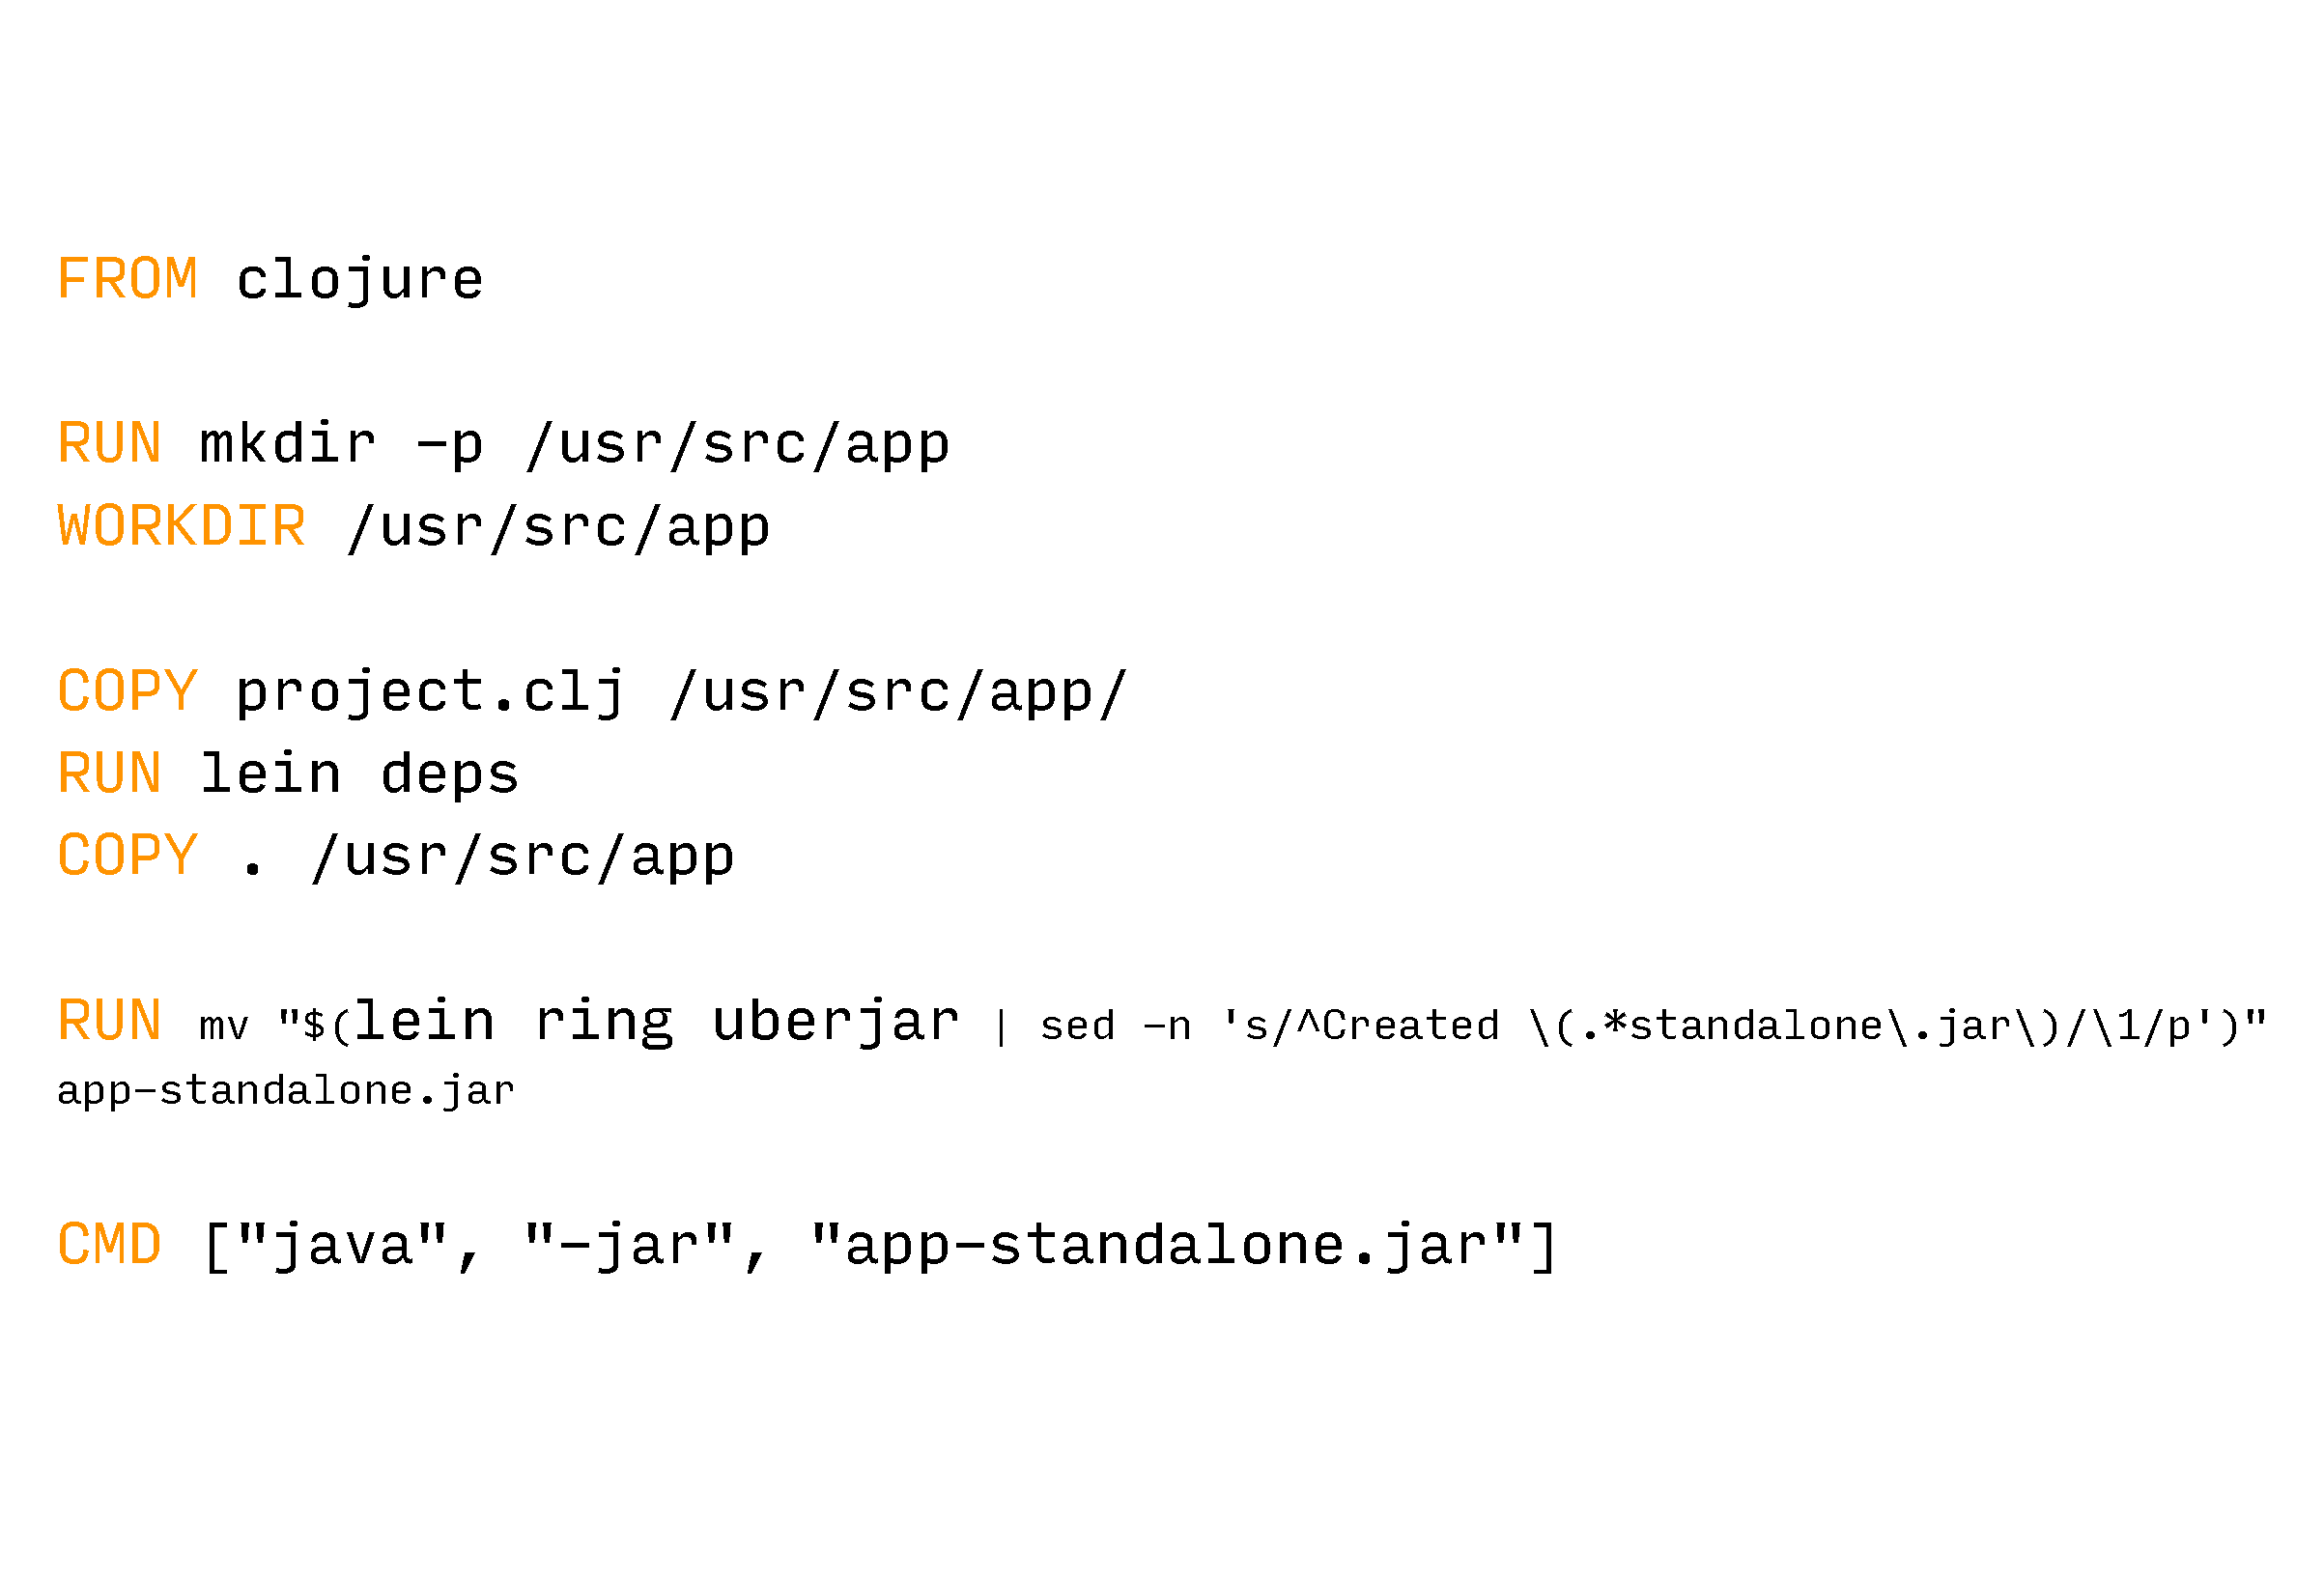
\includegraphics[width=\paperwidth,height=\textheight]{dockerfile.pdf}
%   }
% \end{frame}

% \begin{frame}{Docker-Compose}
%   \begin{itemize}
%     \item Tool zur Unterstützung von Docker-Cli
%     \item Definition von Services als Bestandteil einer App
%     \item Ergänzende Angabe von Konfigurations-Parametern an Containern: Volume-Mounts, Ports, Env-Vars, Netzwerke,..
%     \item Muss sonst bei \texttt{docker exec} Command angegeben werden
%     \item Getrennte Environments für Dev, Test, Prod: \texttt{docker-compose[.dev].yml}
%     \item Zentrale Dokumentation!
%   \end{itemize}
% \end{frame}

\section{Inspirationen für ein UI}
\begin{frame}{Cloud-IDEs}
  \begin{columns}
    \column{.5\textwidth}
    \begin{itemize}
      \item Cloud 9
      \item Source Lair
      \item Eclipse Che
      \item ...
    \end{itemize}

    \column{.5\textwidth}
    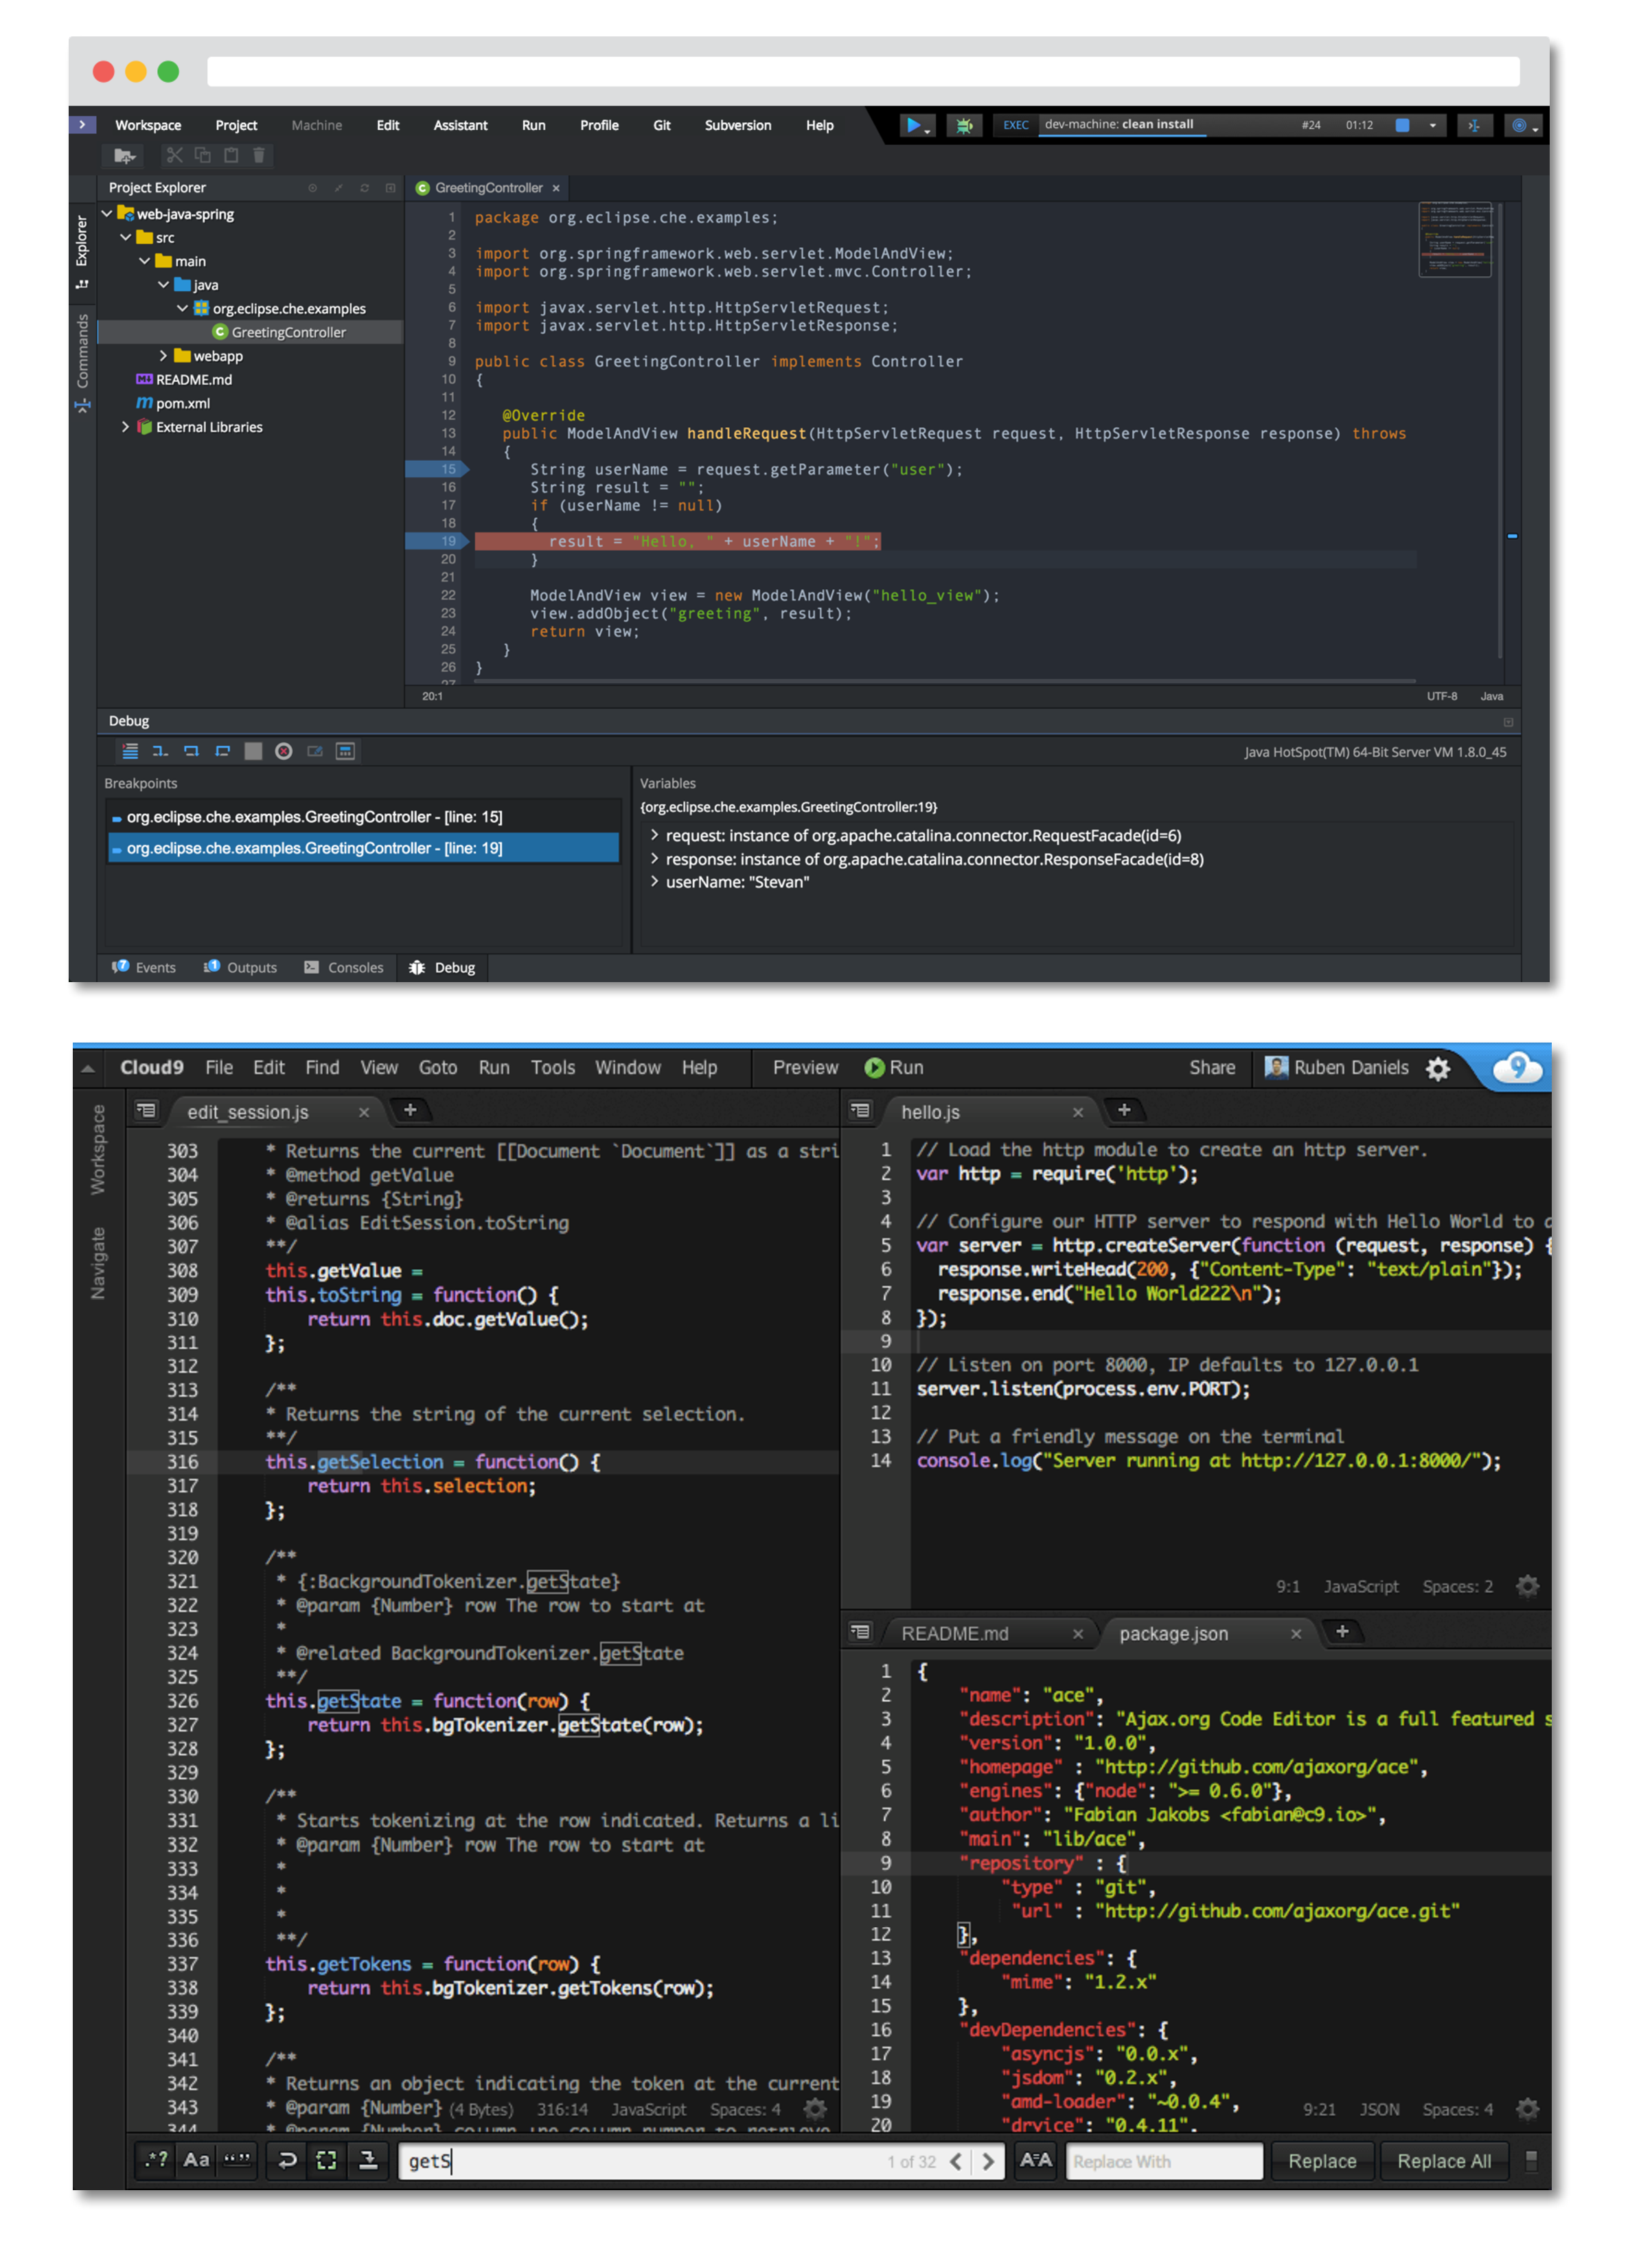
\includegraphics[width=\textwidth]{eclipse.pdf}
  \end{columns}
\end{frame}
\begin{frame}{Tmux Panes}

  % \AddToShipoutPictureFG*{%
  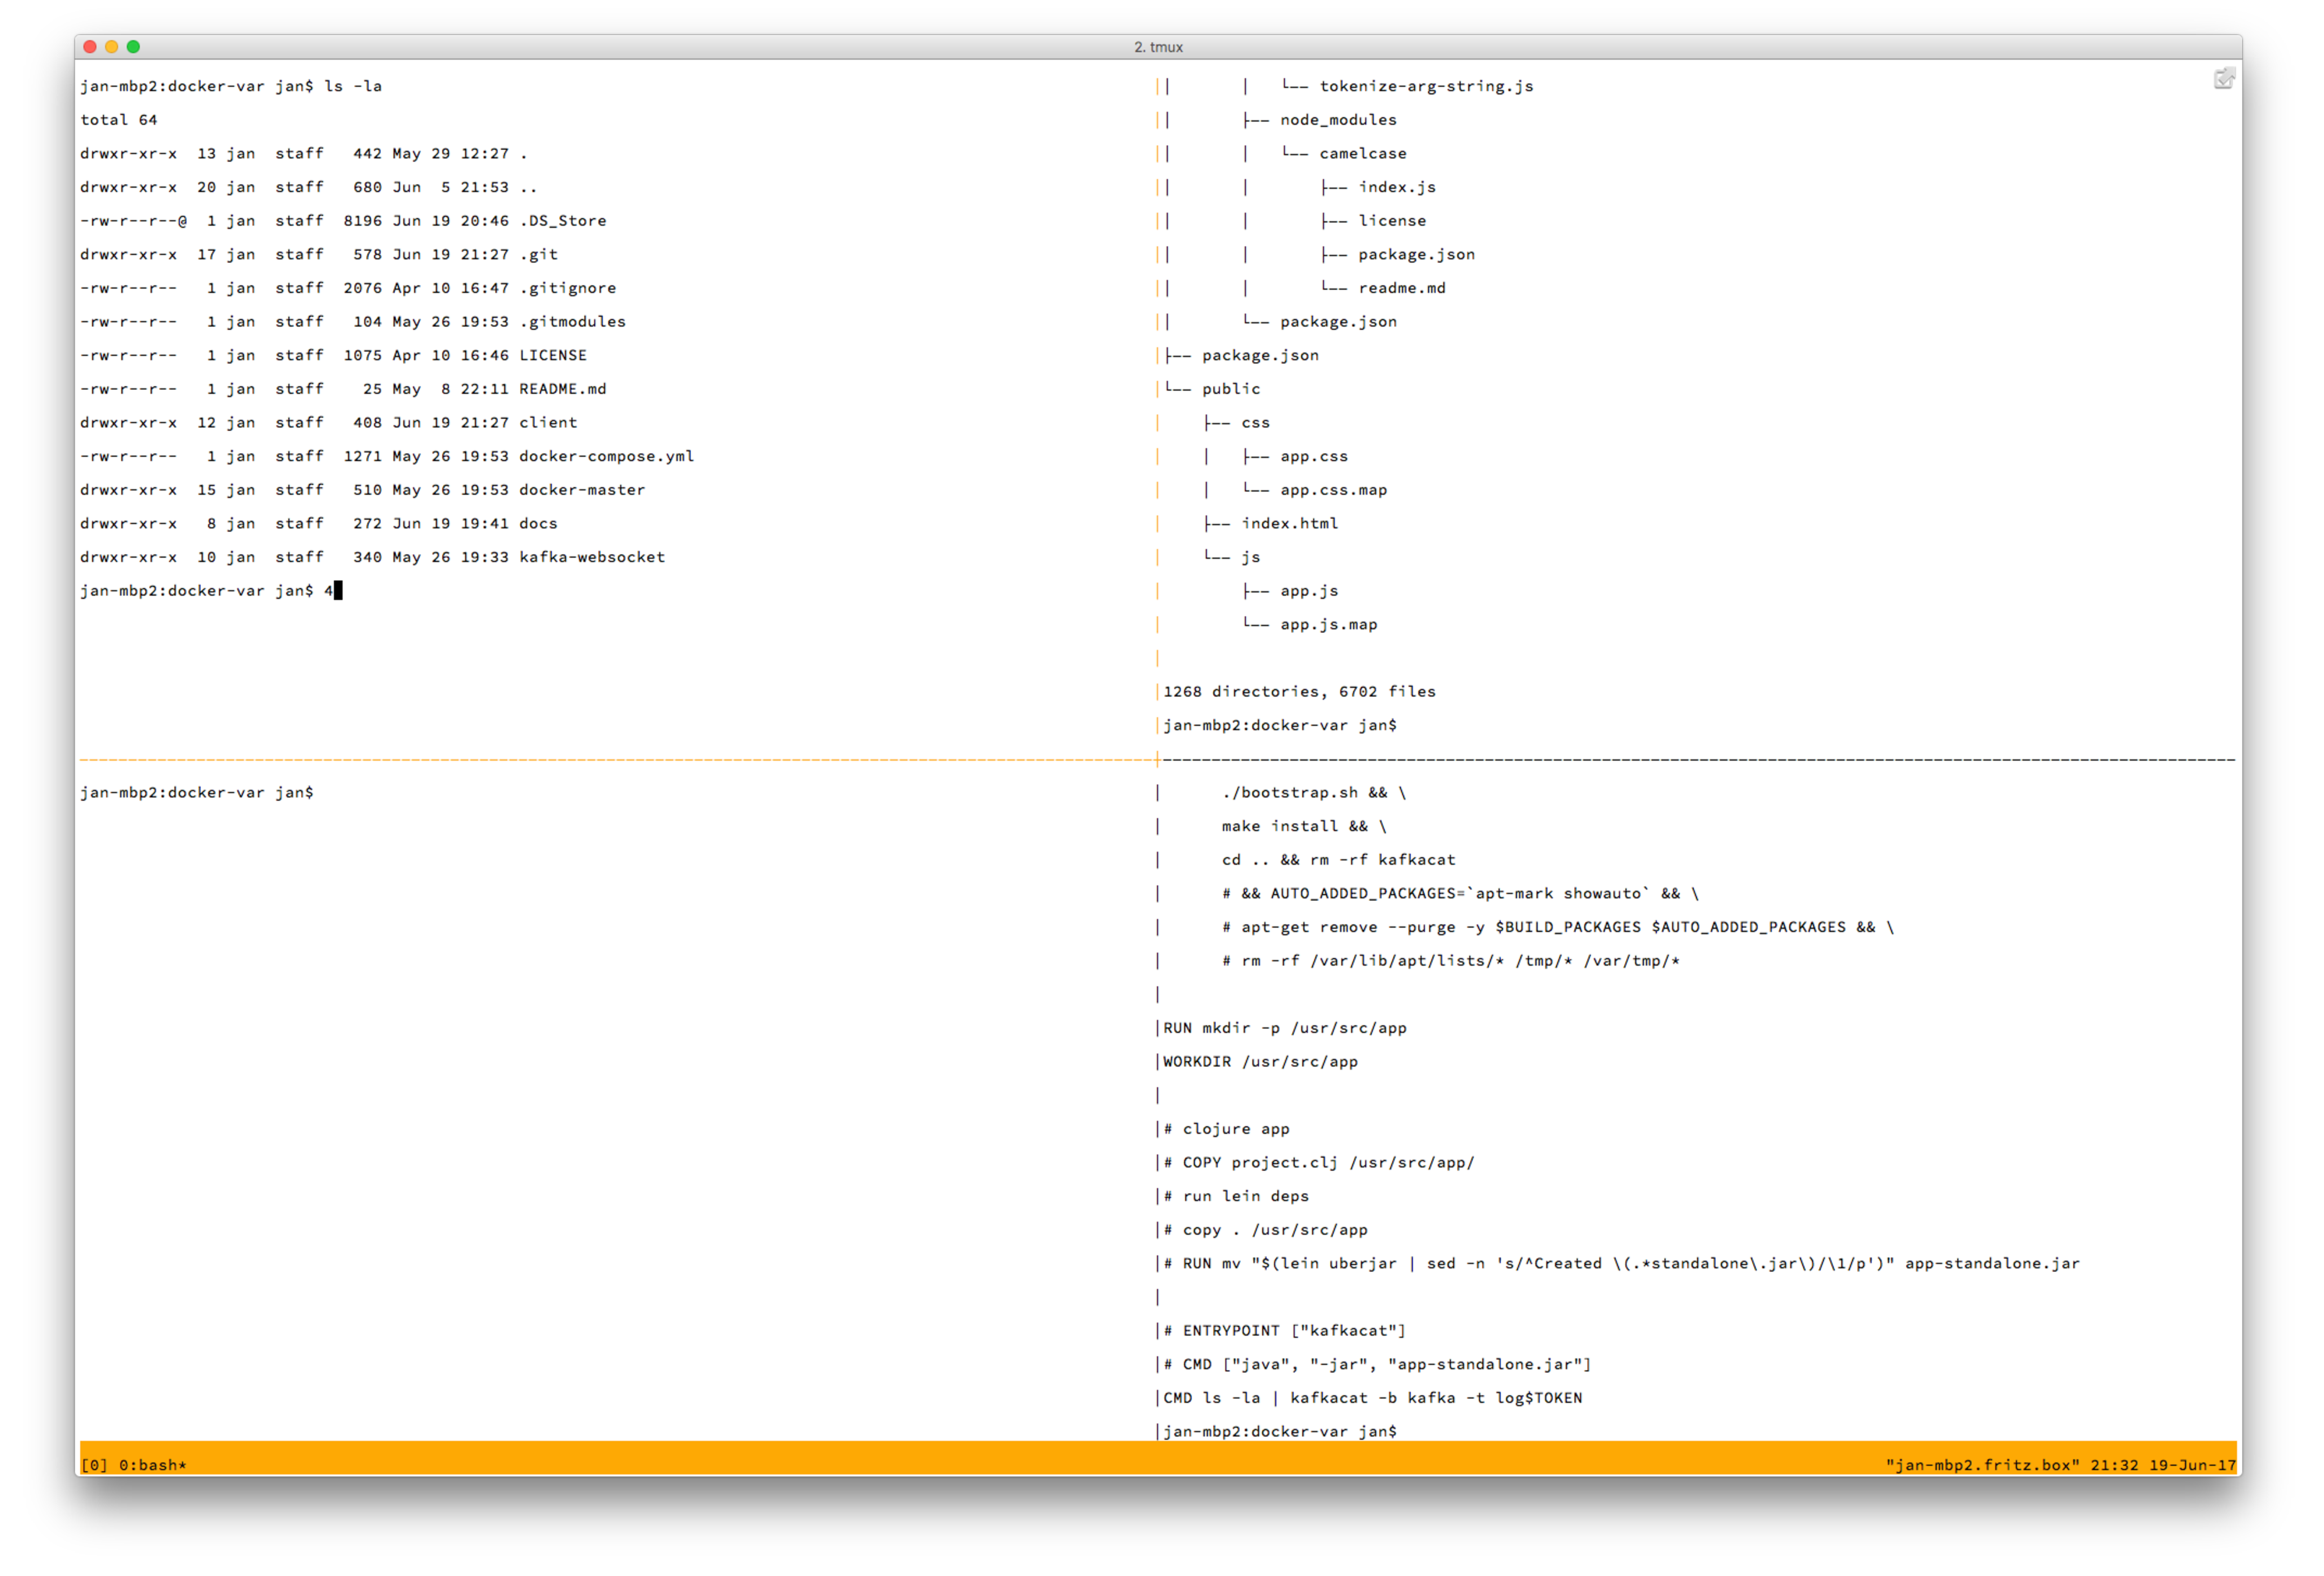
\includegraphics[width=\textwidth]{tmux.pdf}
  % }
\end{frame}
\begin{frame}{xterm.js}
  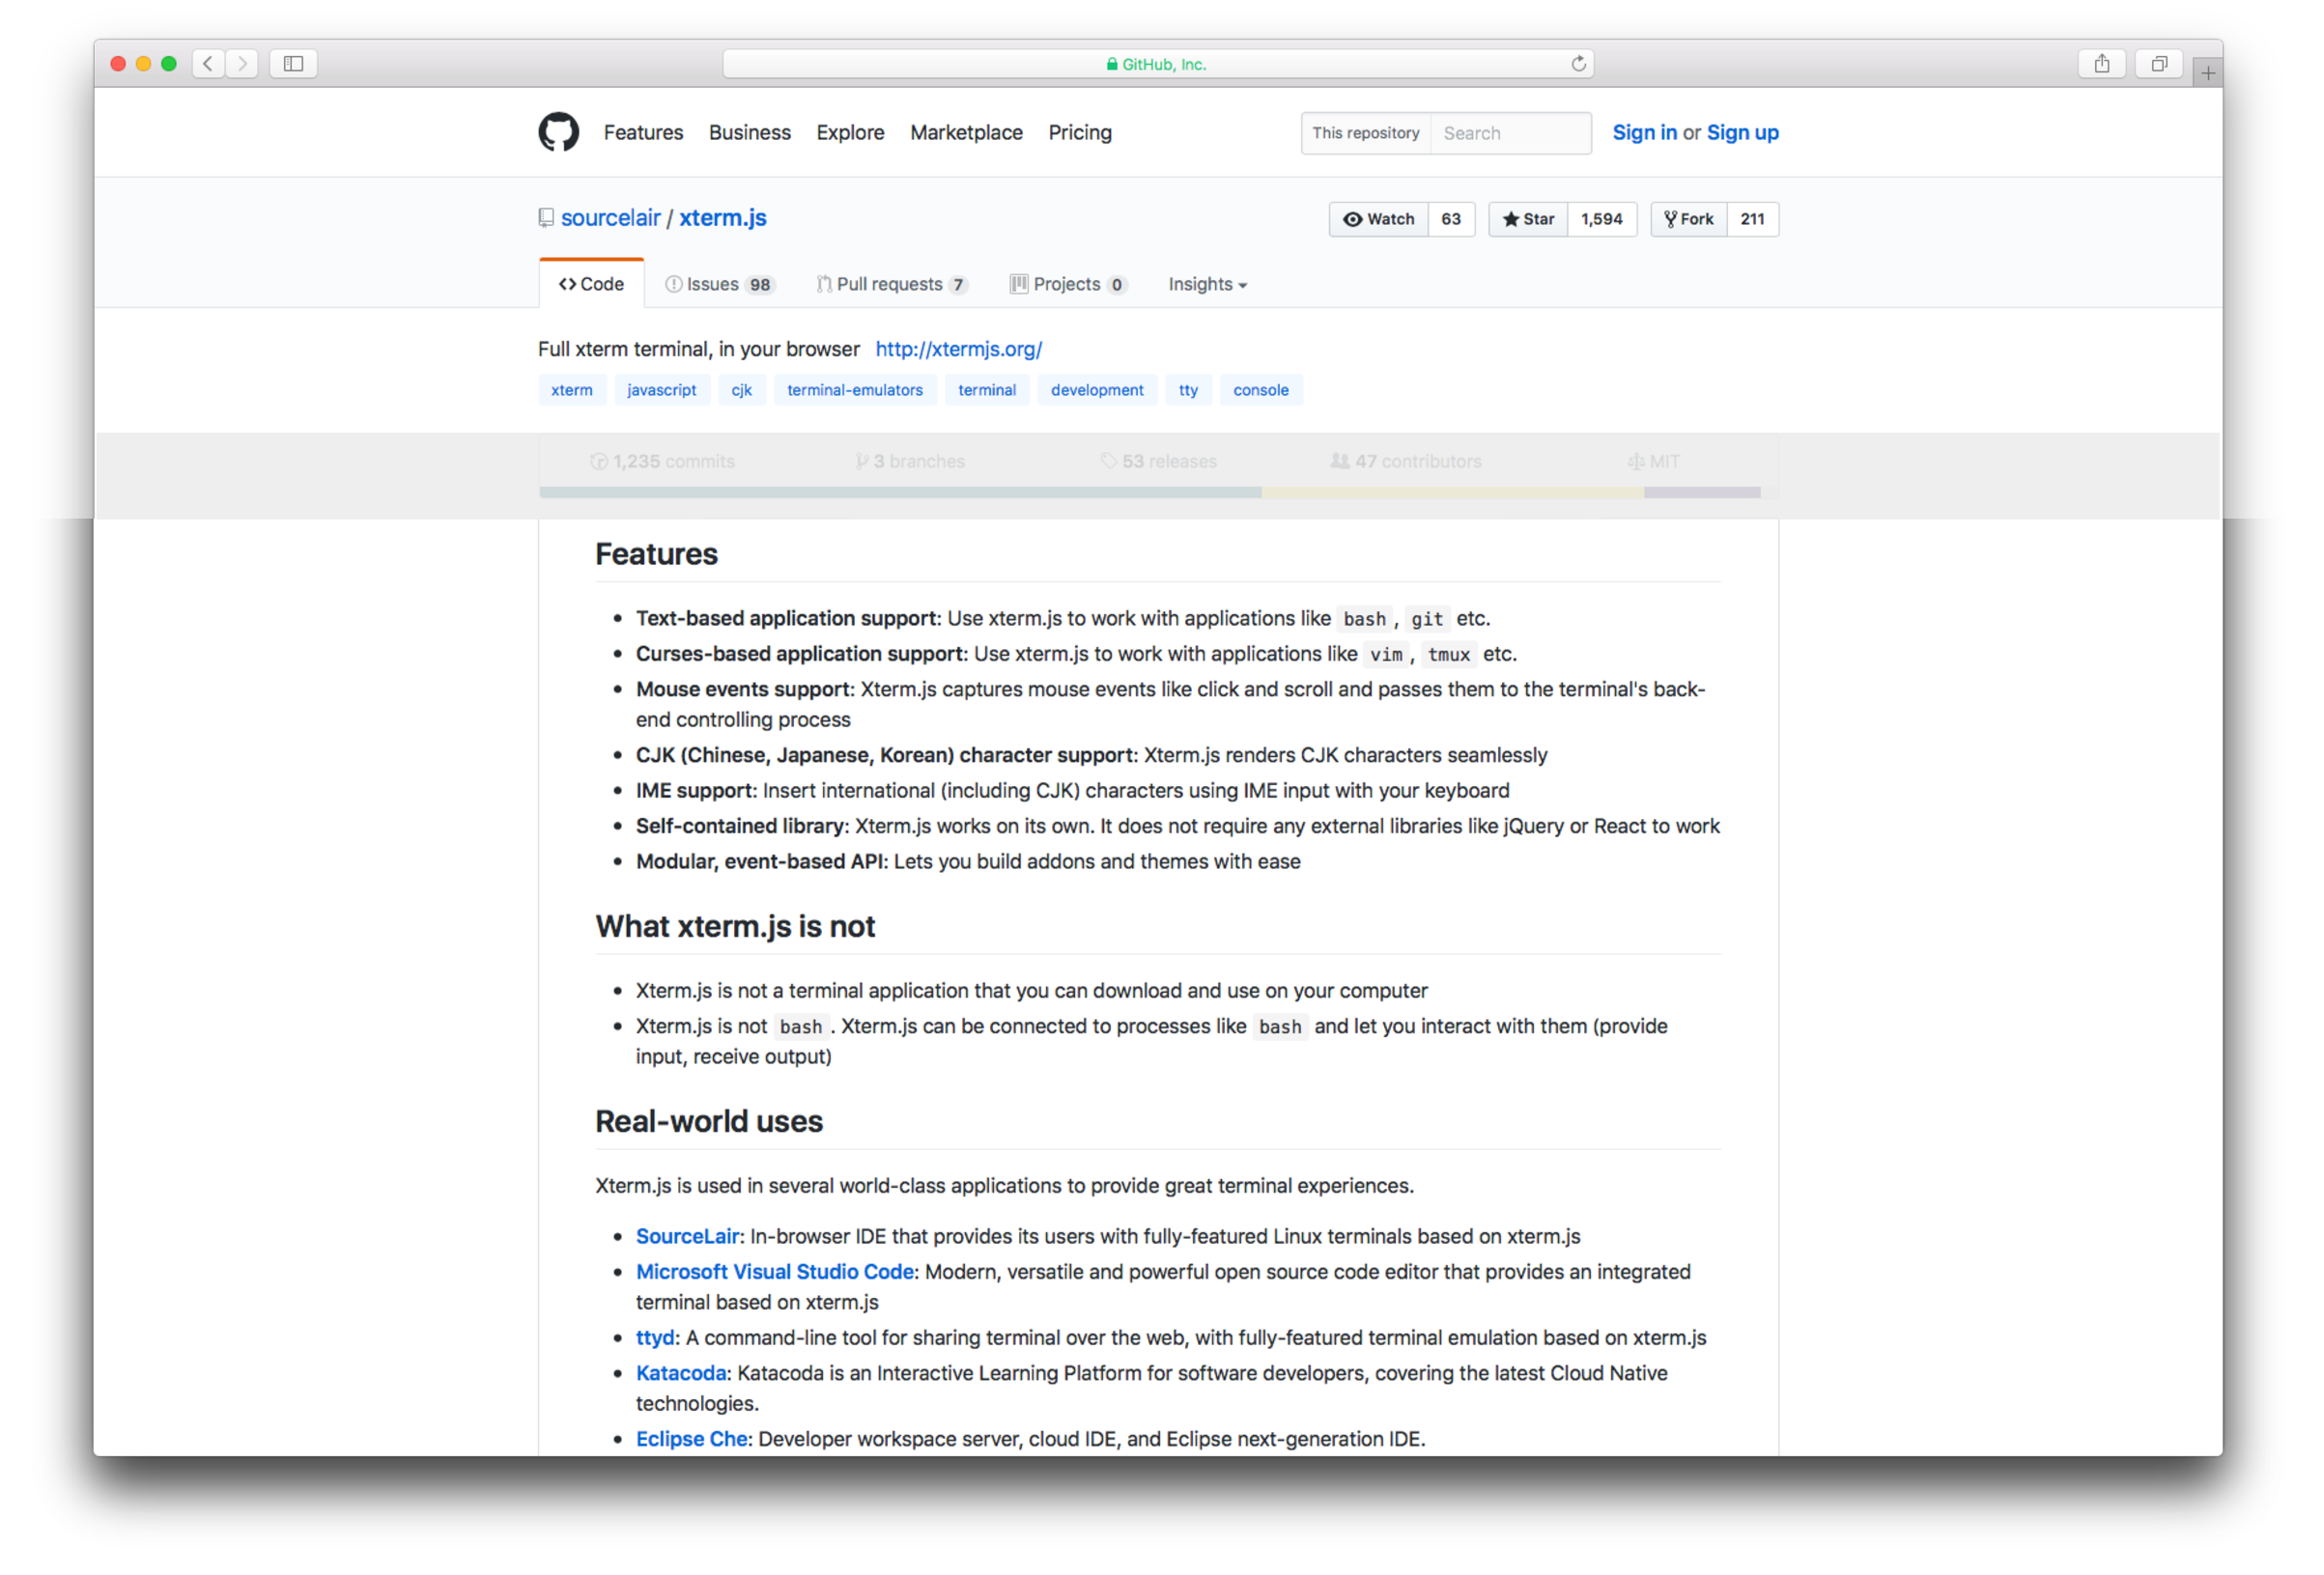
\includegraphics[width=\textwidth]{xterm.pdf}
\end{frame}
\begin{frame}{ttyd}
  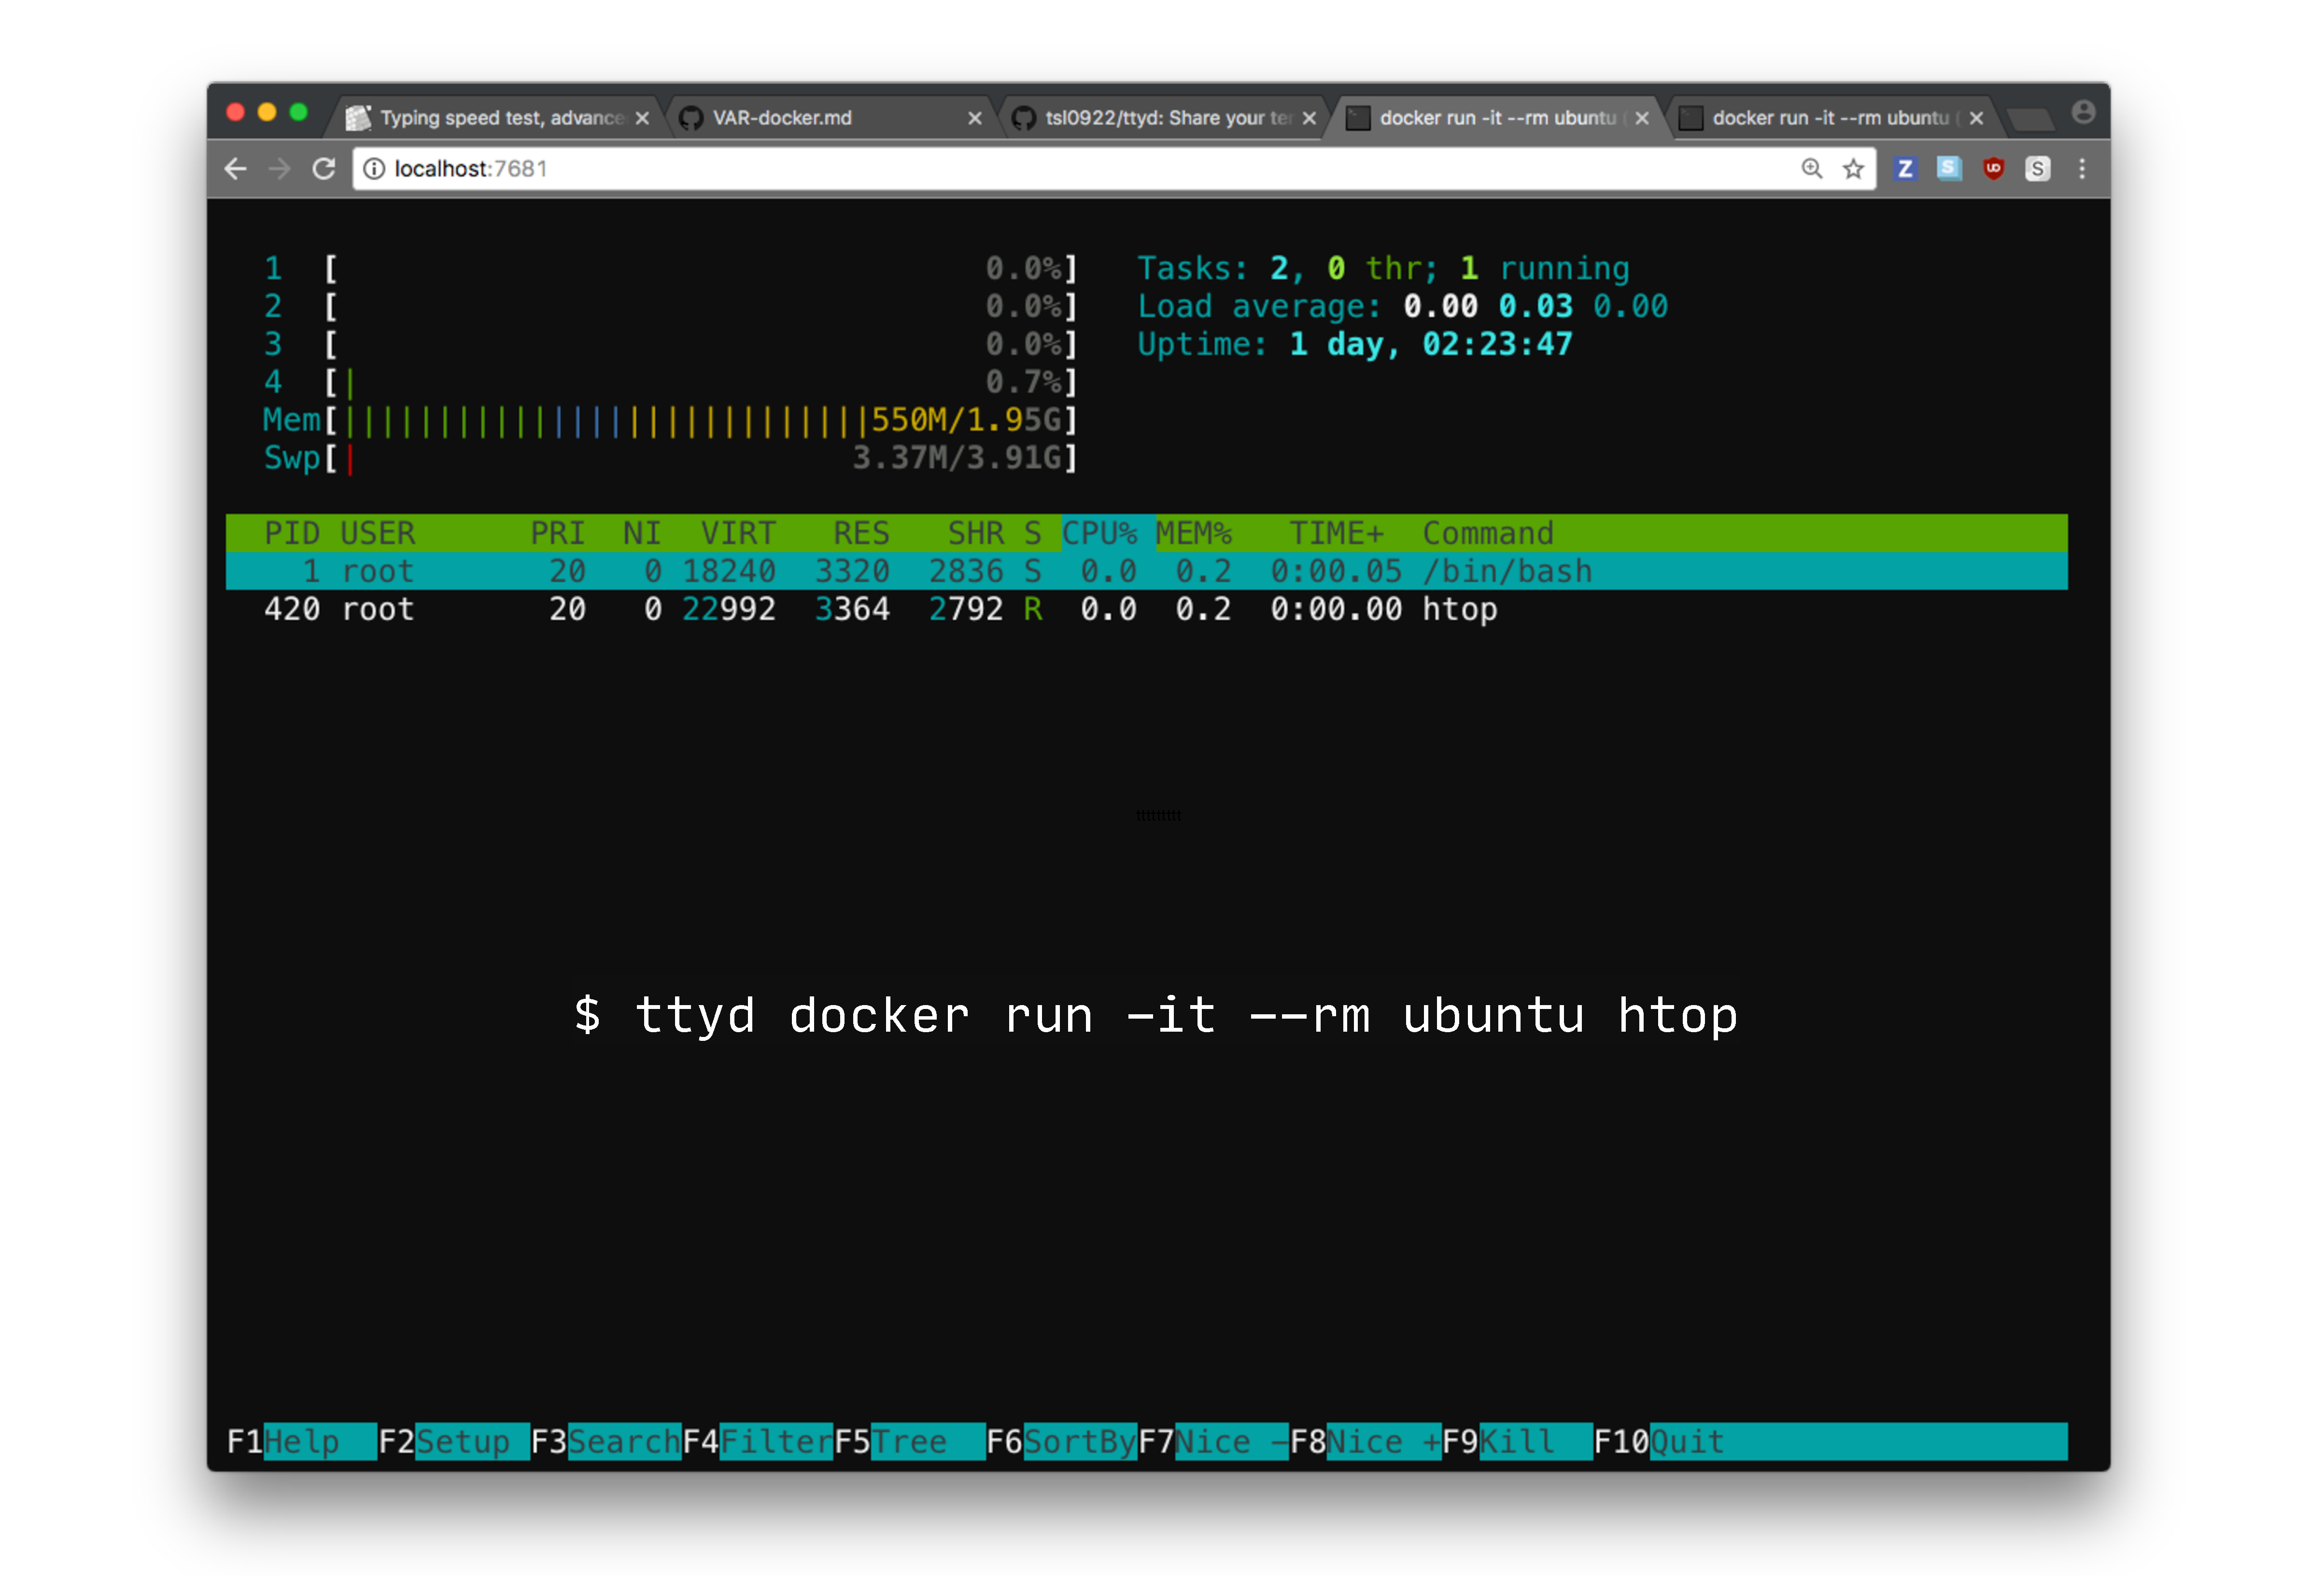
\includegraphics[width=\textwidth]{ttyd.pdf}
\end{frame}

\begin{frame}{Prozess}
  \begin{itemize}
    \item Recherche
    \item Paper-Scribbles
    \item HighFi-Mockups
    \item Implementierung als granulare Funktionen in Elm
      \begin{itemize}
          \item Components
      %   \item HTML + inline Styles
      %   \item in JS wird von stateless-components gesprochen
      \end{itemize}
  \end{itemize}
\end{frame}

\section{„VAR-Tool“}
% \begin{frame}{}
%   \AddToShipoutPictureFG*{%
%     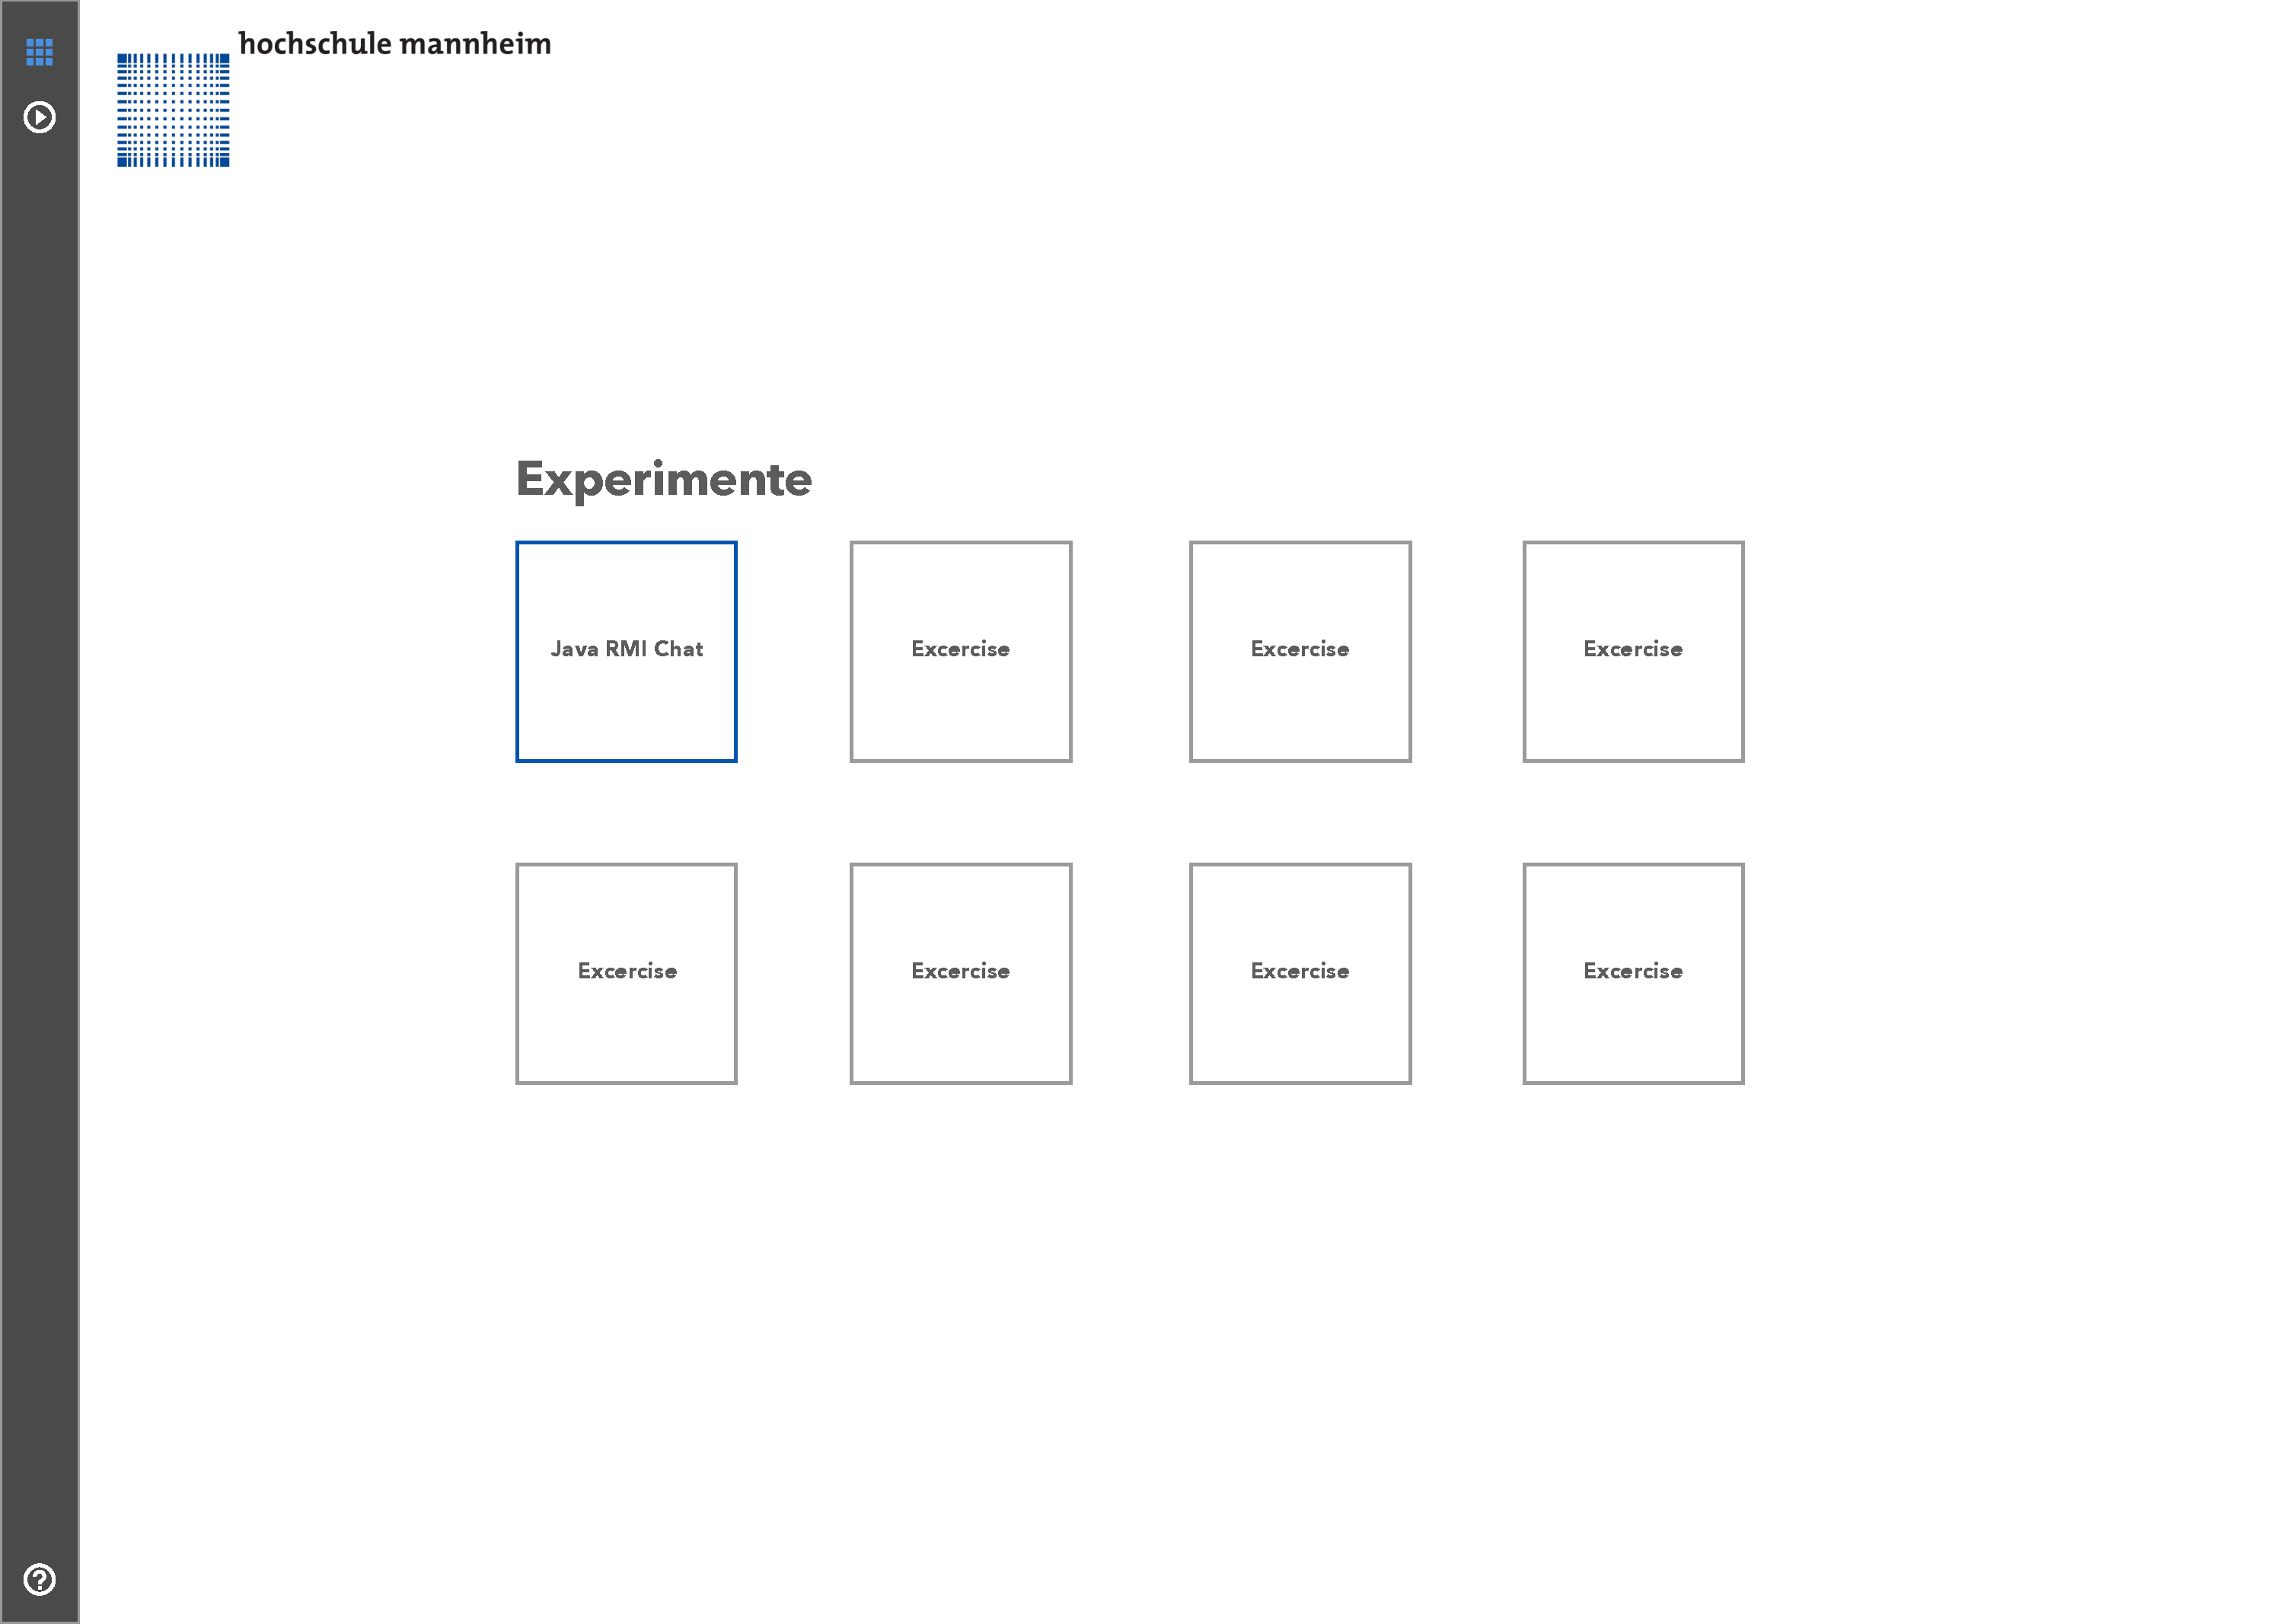
\includegraphics[width=\paperwidth,height=\paperheight,page=1]{ui-mockup.pdf}
%   }
% \end{frame}
% \begin{frame}{}
%   \AddToShipoutPictureFG*{%
%     \includegraphics[width=\paperwidth,height=\paperheight,page=2]{ui-mockup.pdf}
%   }
% \end{frame}
\begin{frame}{Network}
  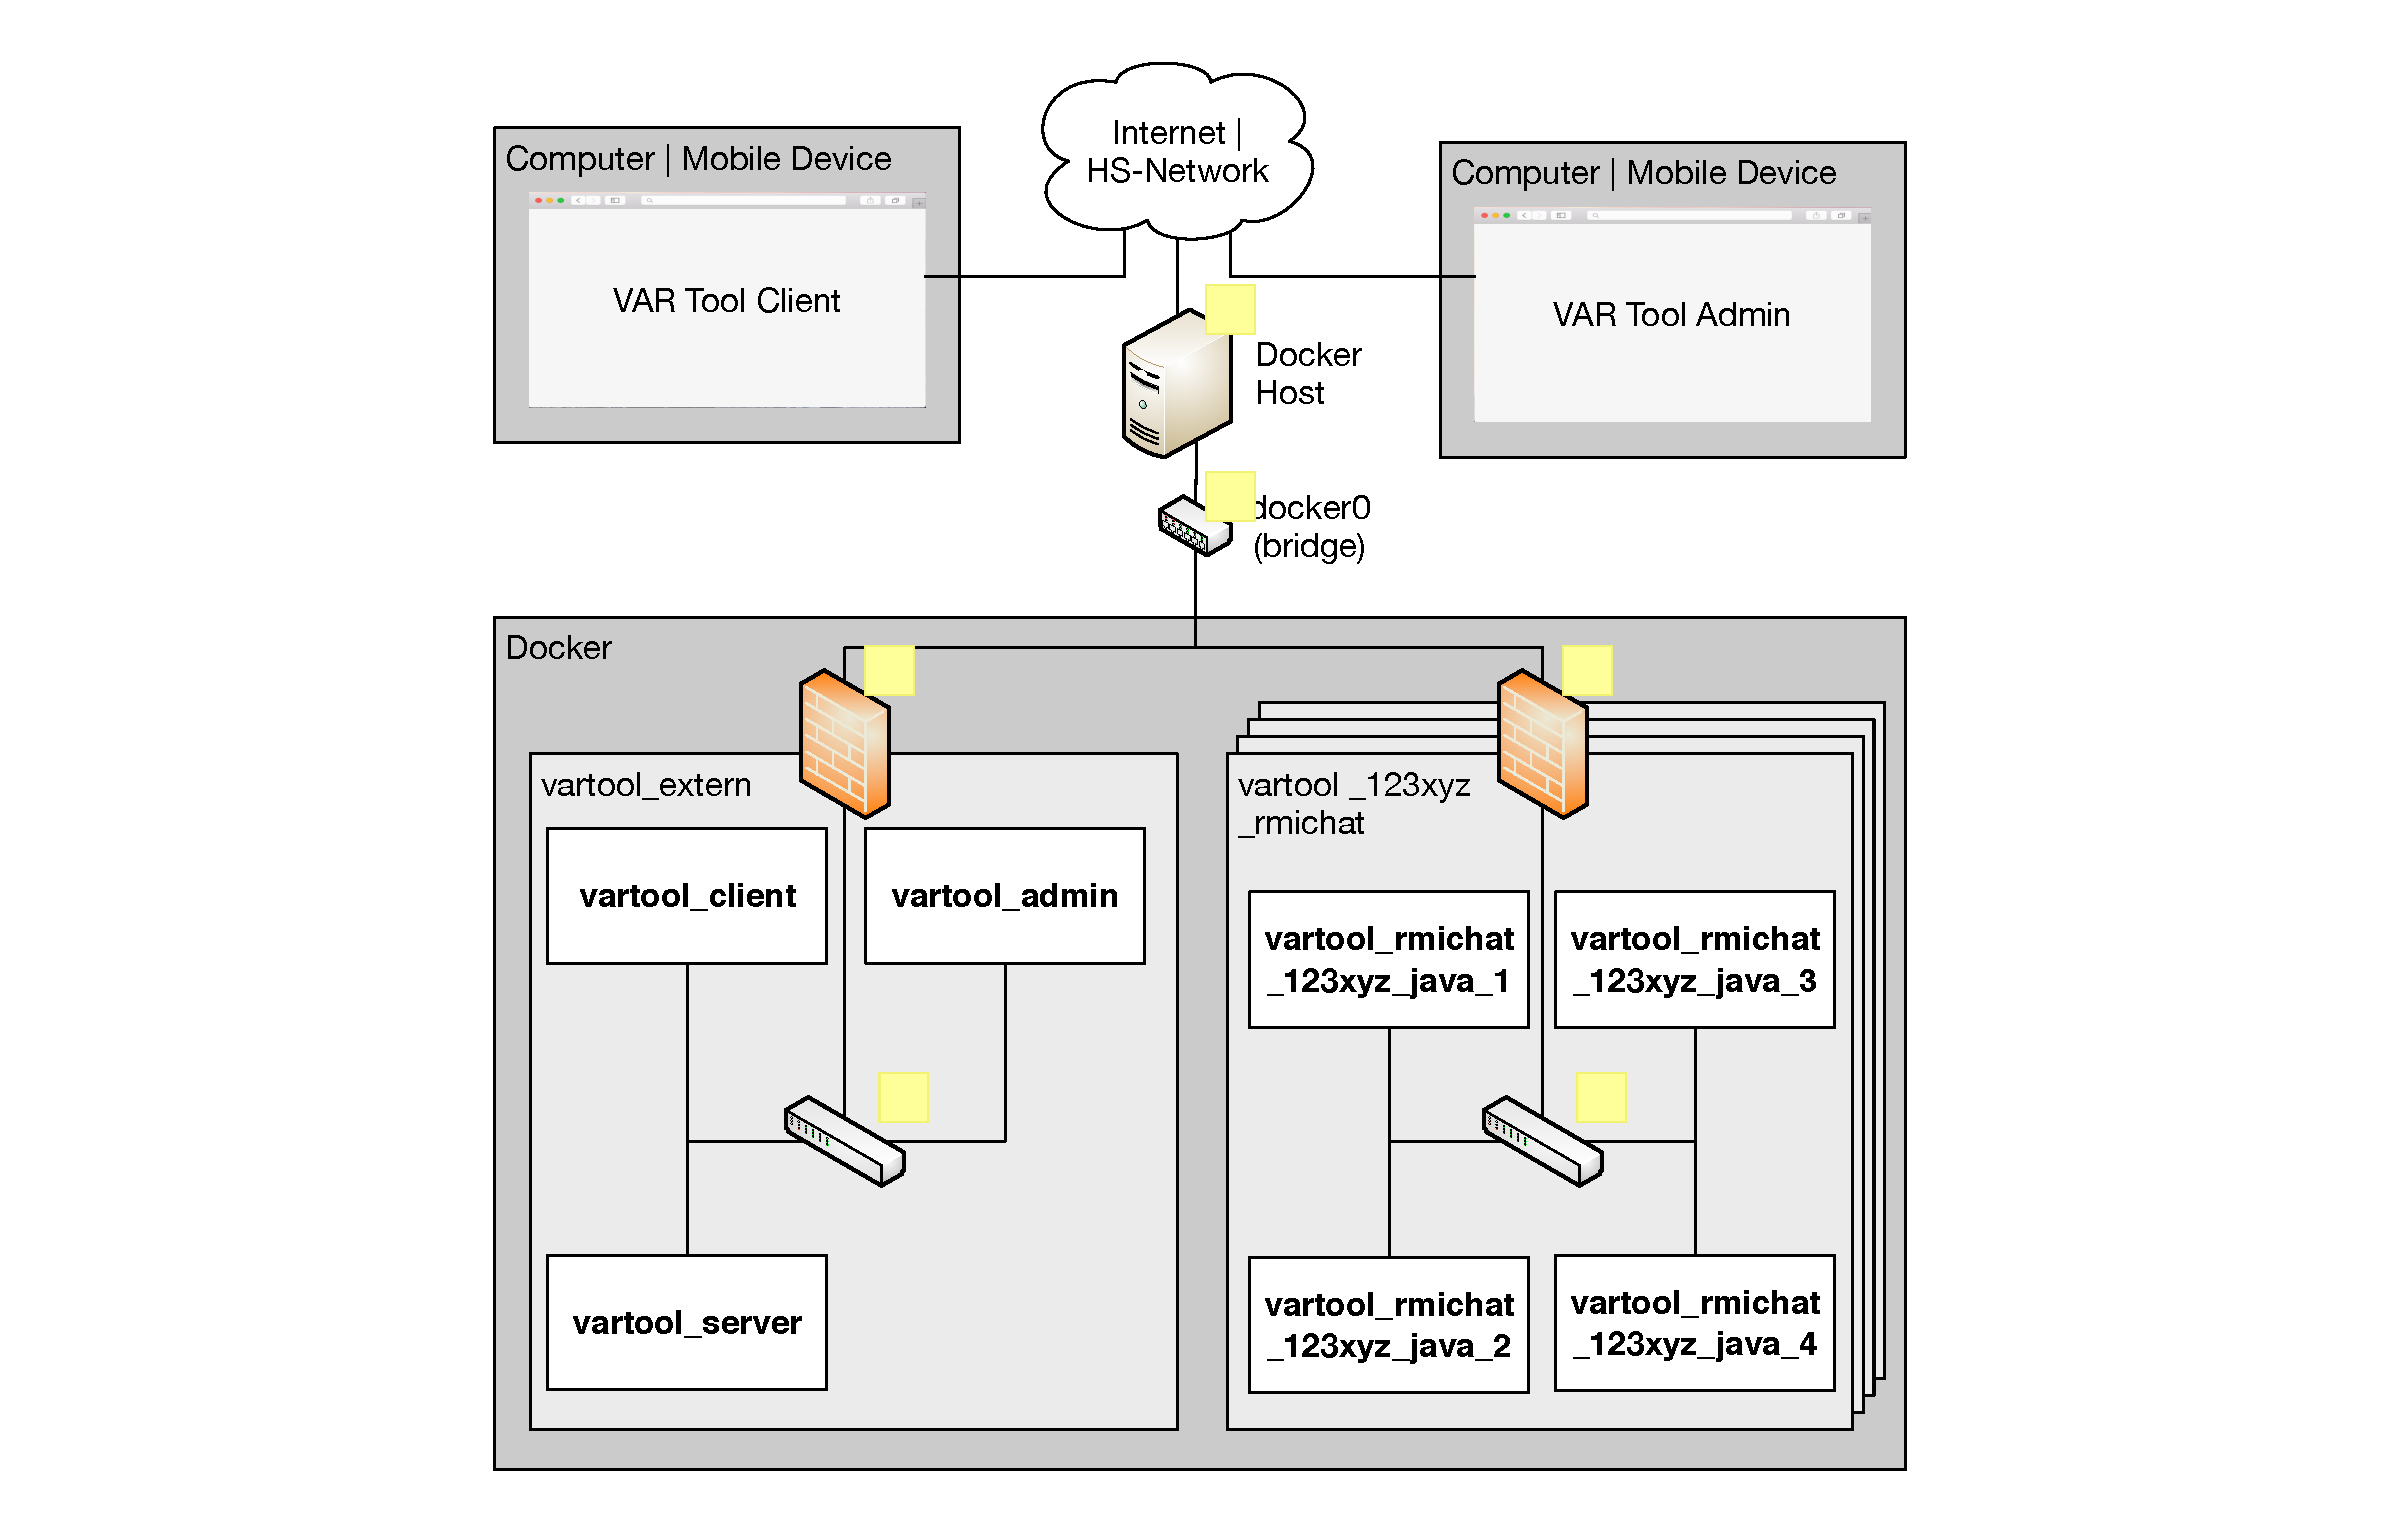
\includegraphics[width=\textwidth]{network_centered.pdf}
\end{frame}
\begin{frame}{State}
  \AddToShipoutPictureFG*{%
    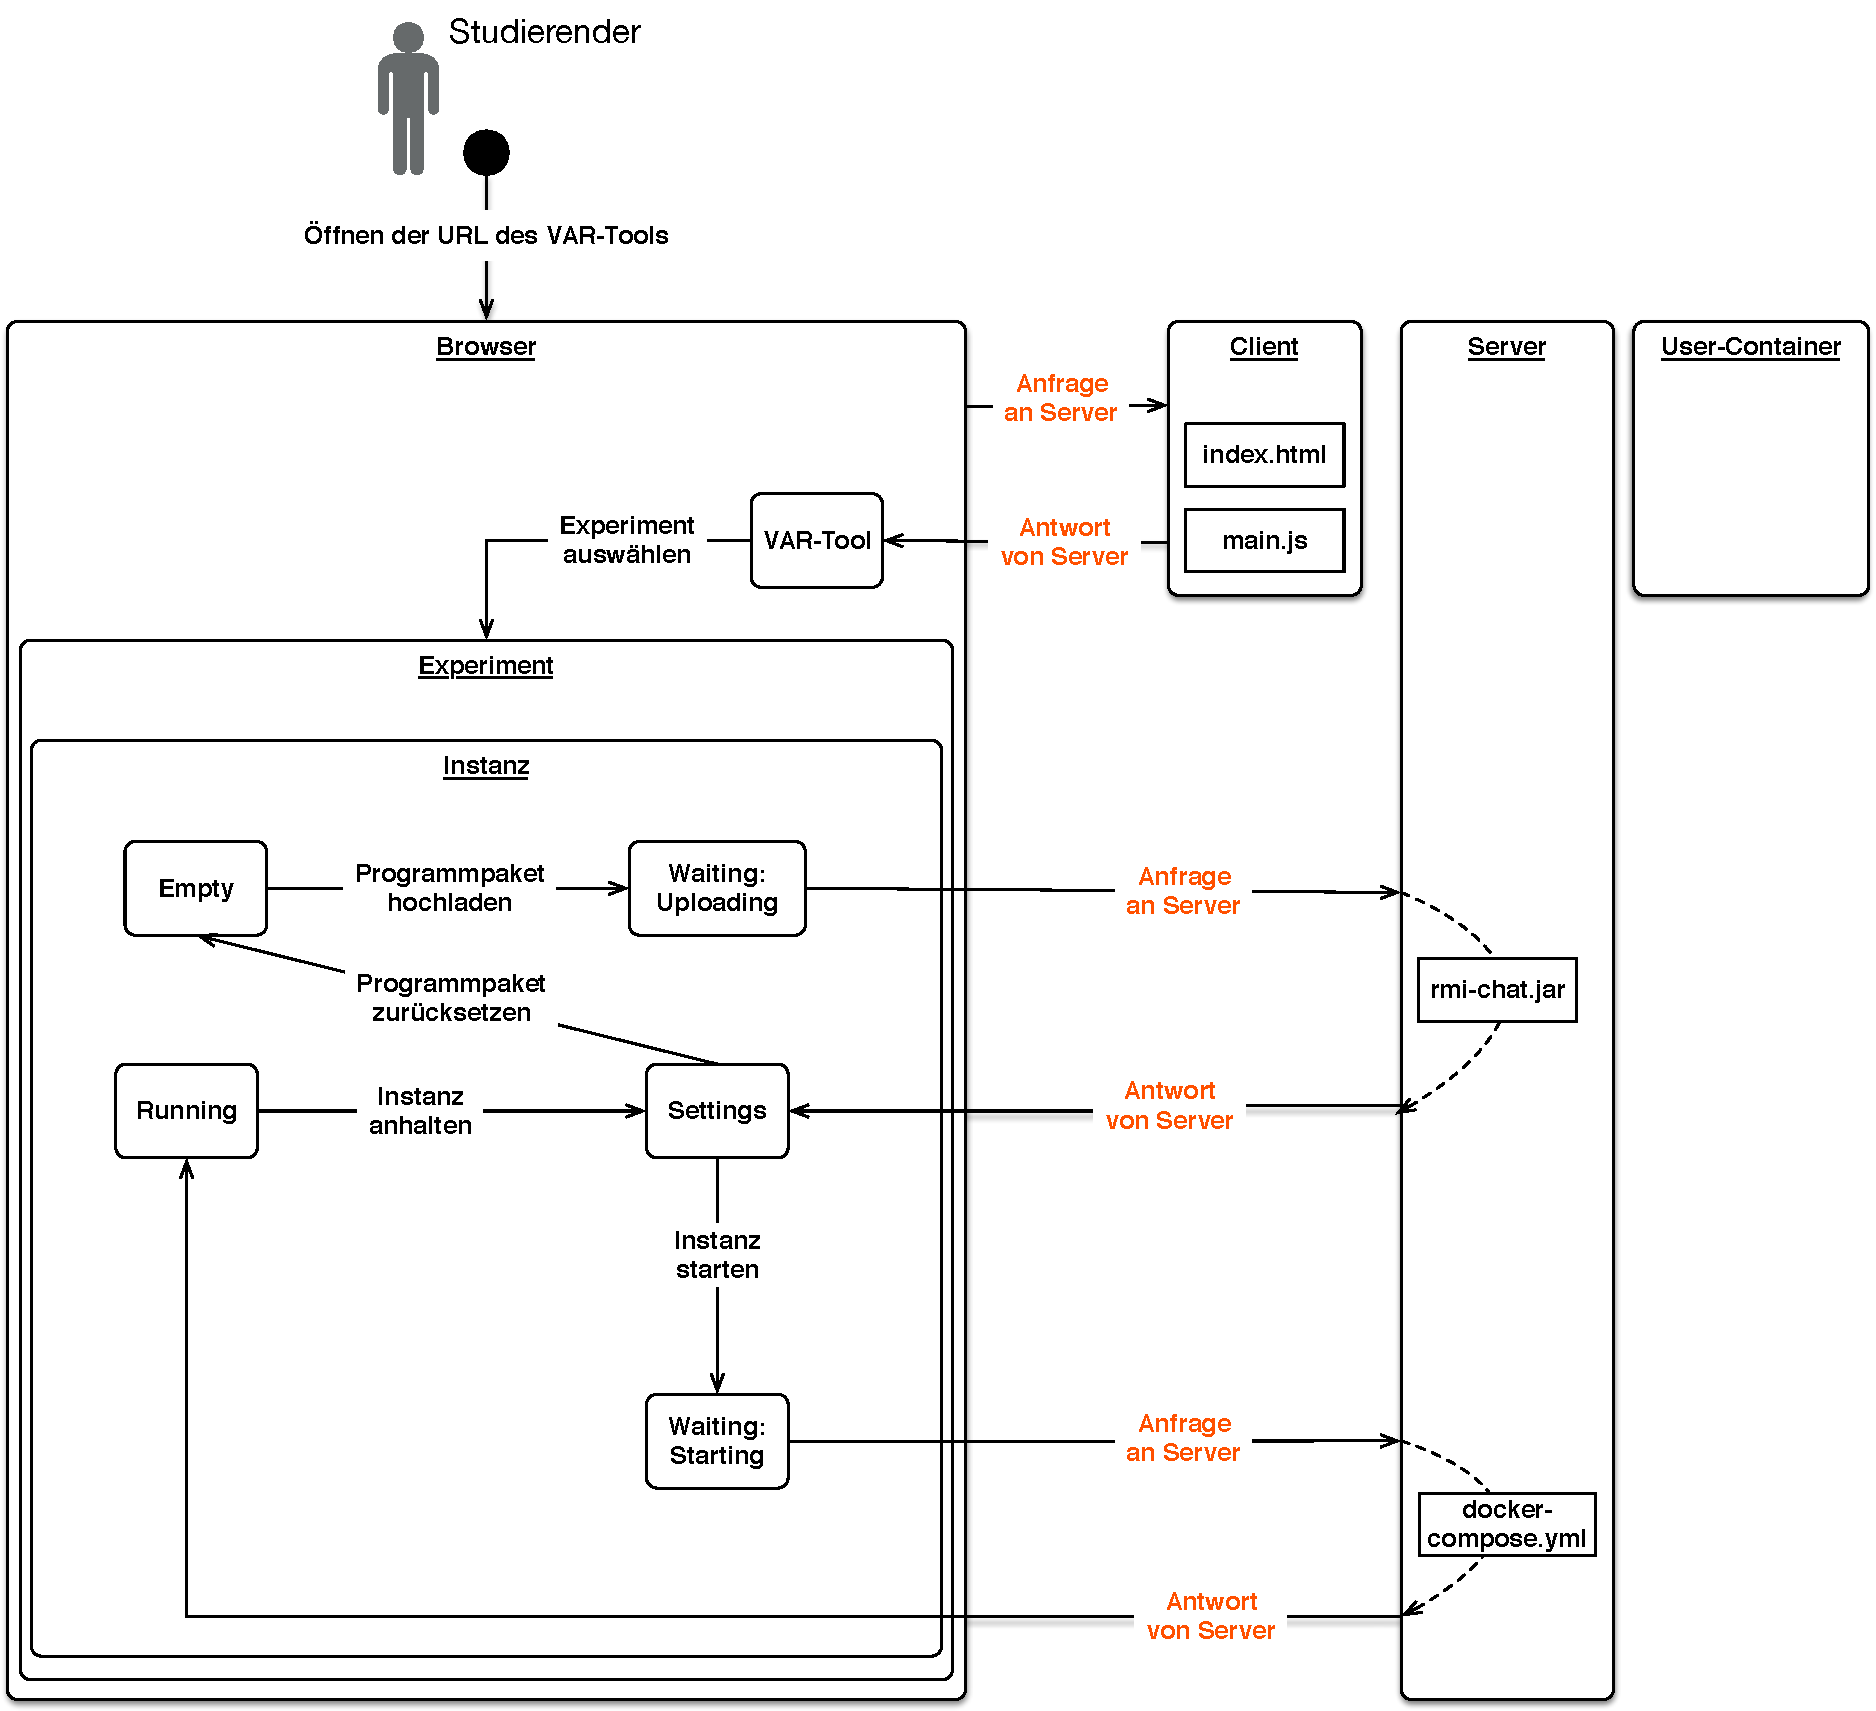
\includegraphics[width=\paperwidth,height=\textheight]{states.pdf}
  }
\end{frame}
\begin{frame}{Deployment}
  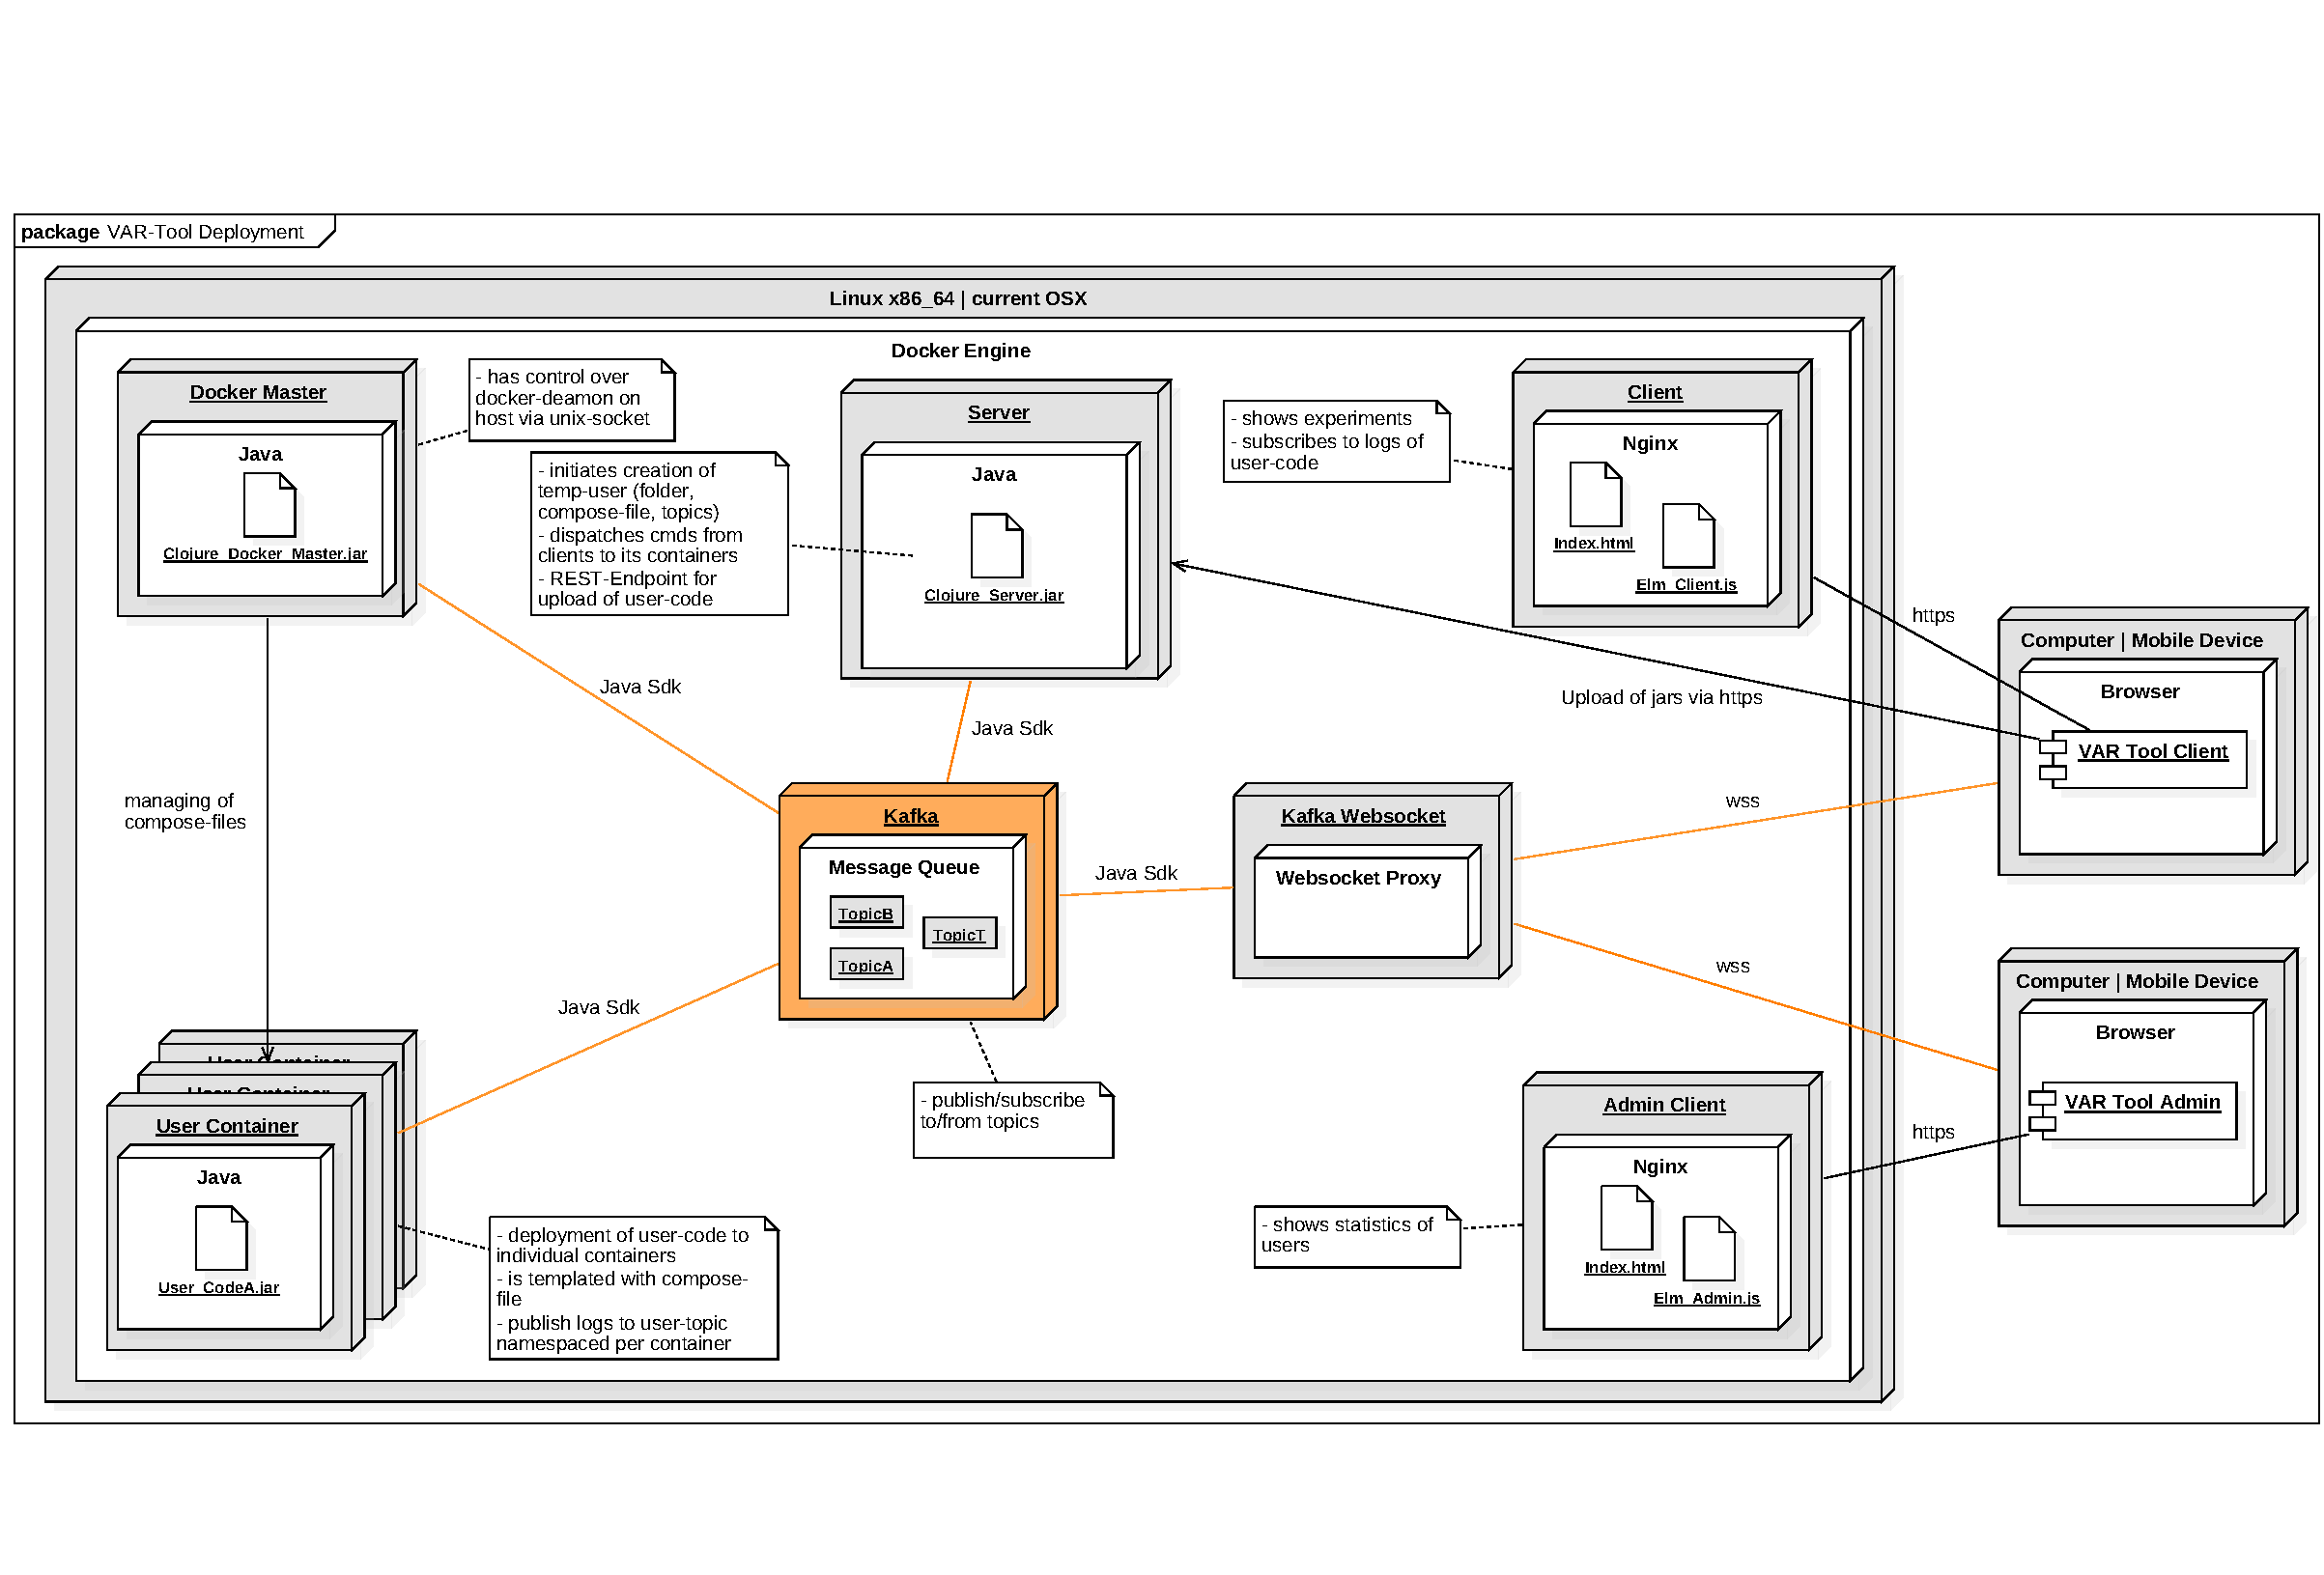
\includegraphics[width=\textwidth]{deployment.pdf}
\end{frame}
% \begin{frame}{Compose-File}
%   \AddToShipoutPictureFG*{%
%     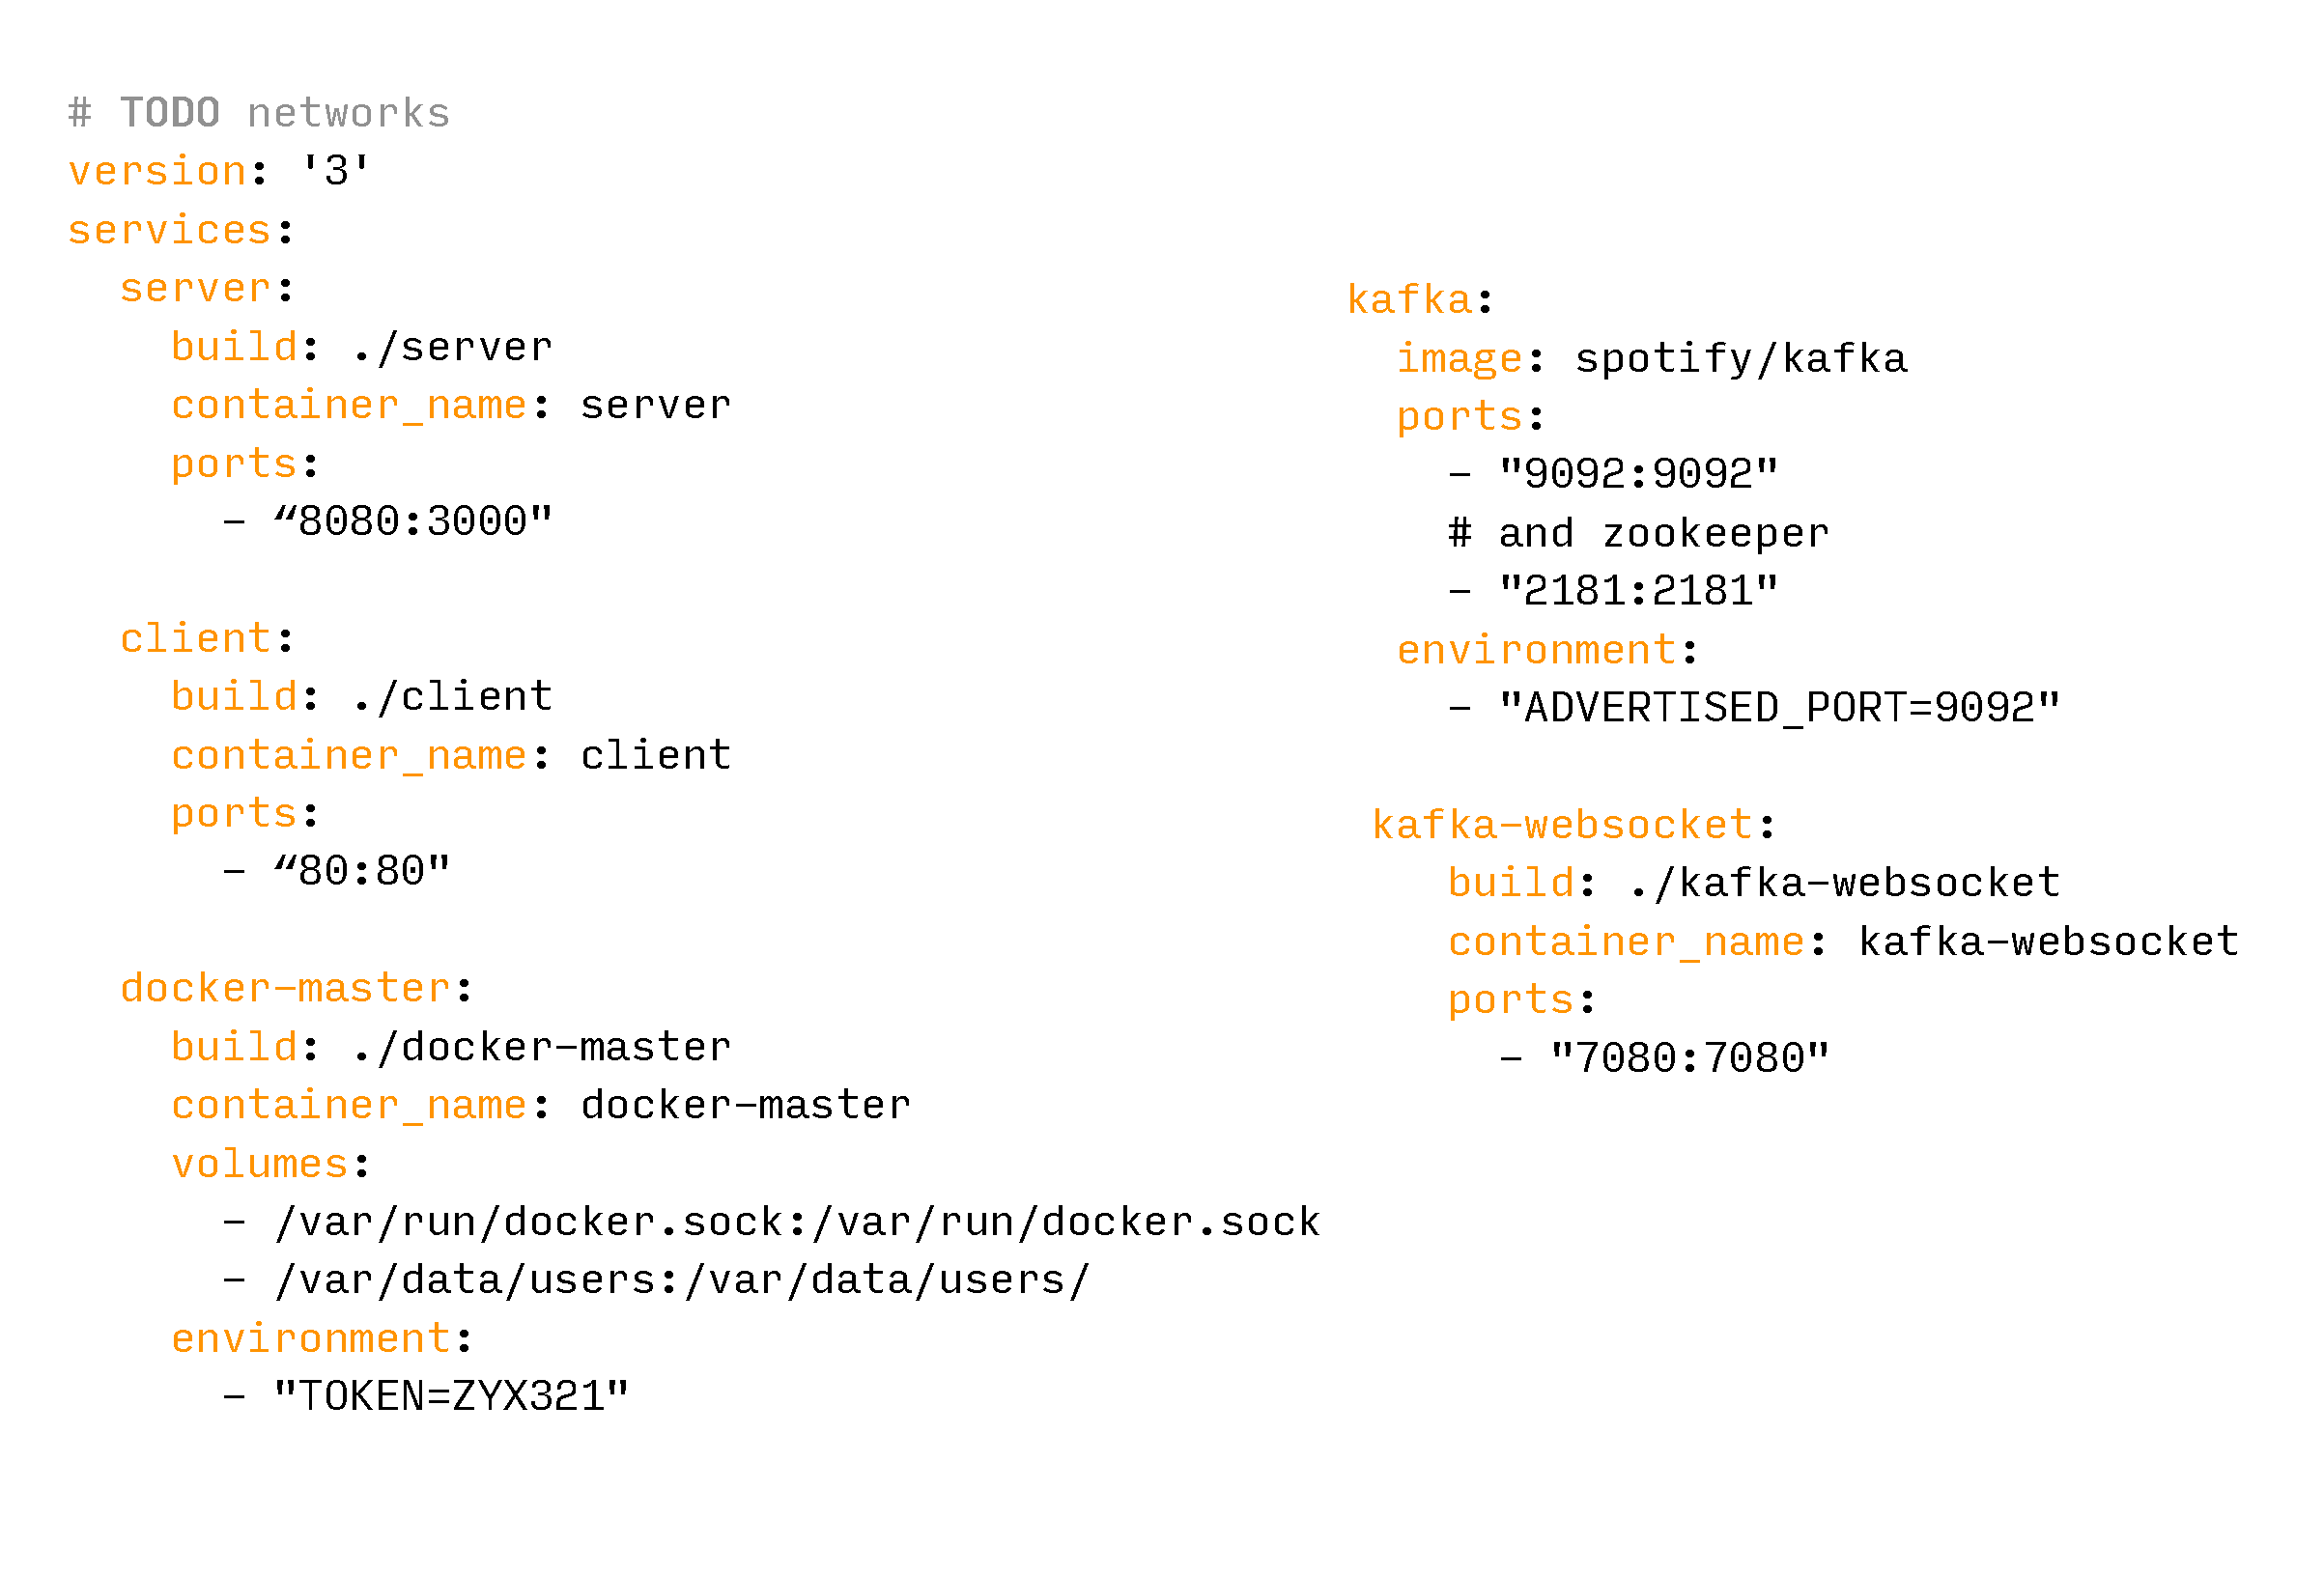
\includegraphics[width=\paperwidth,height=\textheight]{compose.pdf}
%   }
% \end{frame}
\section{Design-Entscheidungen}
\begin{frame}{Design-Entscheidung (1/5)}
  \textbf{Docker als Infrastruktur-Layer}
  \hfill
  → Entscheidung: {\color{green} gut}
  \begin{itemize}
    \item Vorgabe von Prof. Leuchter
    \item Zusätzlich: App in Docker, statt VM
    \item Docker in Docker // Binding von Docker-Socket~\href{https://jpetazzo.github.io/2015/09/03/do-not-use-docker-in-docker-for-ci/}{\color{orange}+}
    \item Problem: Volume-Mount von \texttt{data/} in User-Container leer
      \begin{itemize}
        \item weil Server startende Instanz kann eigener Mount von Host nicht reaktiv weitergeleitet werden (Kopie wäre möglich)
      \end{itemize}
    \item Integration von User-Container und Server über Docker-Daemon
      \begin{itemize}
        \item Bestehende Clojure- oder Java-Sdk-Clients ungeeignet
        \item Curl als Shell-Command
      \end{itemize}
  \end{itemize}
\end{frame}


\begin{frame}{Design-Entscheidung (2/5)}
  \textbf{Trennung von Front- und Backend}
  \hfill
  → Entscheidung: {\color{green} gut}
  \begin{itemize}
    \item Ermöglicht Austauschbarkeit von jeweiliger Implementierung
    \item Parallele Arbeit möglich, ohne den anderen Service zu verletzen
    \item Back- \& Frontend erfordern eigene Build-Pipelines
    \item Development-Container erleichtern die Integration des Toolings beim Entwickeln
  \end{itemize}
\end{frame}

\begin{frame}{Design-Entscheidung (3/5)}
  \textbf{Eigene Websocket-Implementierung}
  \hfill
  → Entscheidung: {\color{green} gut}
  \begin{itemize}
    \item Ursprünglich war Apache Kafka als Integrations-Punkt gedacht, mit Websocket-Adapter Verbindung zum Browser
      \begin{itemize}
    \item Nur Empfangen, wenig konfigurierbar
  \end{itemize}
    \item Nutzen von fertiger Lib für eine TTY-Verbindung im Browser lässt wenig Platz für eigene Implementierung bzw. Use-Case
    \item Pro TTY bzw. Instanz würde man ohne Customization einen weiteren WS-Channel nutzen
    \item Eigene Lösung ermöglicht die Kommunikation von Server und Client mittels einzelnem Channel
    \item Das Protokoll kann selbst definiert werden
  \end{itemize}
  \vspace*{.1cm}
  \begin{columns}[t]
    \column{.5\textwidth}
    \texttt{\tiny\{ kind: command, \\ subkind: start-instance,
      \\ payload: \{ experimentId: rmichat, \\\hspace*{1cm}instanceId: 1, \\\hspace*{1cm}mainClass: var.rmi.chat.ChatClient, \\\hspace*{1cm}arguments: Anton \}\}}
    \column{.5\textwidth}
    \texttt{\tiny\{ kind: message, \\subkind: log,
      \\ payload: \{ experimentId: rmichat, \\\hspace*{1cm}instanceId: 1, \\\hspace*{1cm}log: Hello\}\}}
  \end{columns}
\end{frame}


\begin{frame}{Design-Entscheidung (4/5)}
  \textbf{Elm für Frontend}
  \hfill
  → Entscheidung: {\color{green} gut}
  \begin{itemize}
    \item Szenario passend für Single-Page-Application (SPA)
    \item reaktiv → Virtual DOM
    \item State-Handling mit TEA
    \item rein funktional, Immutable
    \item Websocket als Task mit resultierender Elm-Msg bei Senden und Empfangen auf WS-Channel
    \item Encoding/Decoding von JSON-Strings zu Elm-Types
      \begin{itemize}
        \item Typisiertes Message-Protokoll
      \end{itemize}
  \end{itemize}
\end{frame}

\begin{frame}{Design-Entscheidung (5/5)}
  \textbf{Clojure für Backend}
  \hfill
  → Entscheidung: {\color{yellow} mittelmäßig}
  \begin{itemize}
    \item Lisp macht Spaß
    \item Ring-Implementierung erwies sich als problematisch :(
      \begin{itemize}
        \item CSRF-Token trotz Nutzen von API-Settings
        \item Reihenfolge von Ring-Handlern entscheidend
      \end{itemize}
    \item JSON-Encoding \& -Decoding war durch Lib sehr einfach
    \item Bestehendes JAVA-Ecosystem: bspw. UUID
    \item Abstraktion des Websocket-Handlers von Http-Kit war hilfreich
      \begin{itemize}
        \item State-Machine
      \end{itemize}
    \item Immutable :)
  \end{itemize}
\end{frame}

\begin{frame}{Fazit \& Ausblick}
  \begin{itemize}
    \item Viele Probleme, da Fokus auf Full-Stack
    \item Integration der Komponenten
    \item Üben von Polyglott
  \end{itemize}
  \begin{itemize}
    \item Sehr spannendes Thema
    \item Viel Raum für weitere (studentische) Arbeiten
    \item Erstrebenswerte Aufgabe der Fakultät
  \end{itemize}
\end{frame}

% \begin{frame}[noframenumbering,plain]{Fin}
%   Danke für die Aufmerksamkeit. -- Fragen?
% \end{frame}
\end{document}
